\documentclass[12pt]{article}
\usepackage{graphicx} % Required for inserting images
\usepackage{setspace}
\usepackage{blindtext}
\usepackage{hyperref}
\usepackage{longtable}
\usepackage{amsmath}
\usepackage{float}
\usepackage{booktabs, multirow} % for borders and merged ranges
\usepackage{soul}% for underlines
\usepackage[table]{xcolor} % for cell colors
\usepackage{changepage,threeparttable} % for wide tables
\usepackage{graphicx}
\graphicspath{ {./images/} }
% Styles
% Newcommand
%% Point
\newcommand{\point}[1]{\draw[fill=black] (#1) circle (1.5pt);}
%node [shift={(#3)}] {#2};

% Style

\usepackage{pgfplots}
\pgfplotsset{compat=newest}
\usetikzlibrary{calc}
\usepackage{amssymb}
\usepackage{comment}
 \usepackage[breakable]{tcolorbox}
\usepackage{parskip} % Basic figure setup, for now with no caption control since it's done
    % automatically by Pandoc (which extracts ![](path) syntax from Markdown).
    \usepackage{graphicx}
    % Maintain compatibility with old templates. Remove in nbconvert 6.0


\usepackage{textcomp} % defines textquotesingle
    % Hack from http://tex.stackexchange.com/a/47451/13684:
    \AtBeginDocument{%
        \def\PYZsq{\textquotesingle}% Upright quotes in Pygmentized code
    }
    \usepackage{upquote} % Upright quotes for verbatim code
    \usepackage{eurosym} % defines \euro

    \usepackage{iftex}
    \ifPDFTeX
        \usepackage[T1]{fontenc}
        \IfFileExists{alphabeta.sty}{
              \usepackage{alphabeta}
          }{
              \usepackage[mathletters]{ucs}
              \usepackage[utf8x]{inputenc}
          }
    \else
        \usepackage{fontspec}
        \usepackage{unicode-math}
    \fi

    \usepackage{fancyvrb} % verbatim replacement that allows latex
    \usepackage{grffile} % extends the file name processing of package graphics
                         % to support a larger range
    \makeatletter % fix for old versions of grffile with XeLaTeX
    \@ifpackagelater{grffile}{2019/11/01}
    {
      % Do nothing on new versions
    }
    {
      \def\Gread@@xetex#1{%
        \IfFileExists{"\Gin@base".bb}%
        {\Gread@eps{\Gin@base.bb}}%
        {\Gread@@xetex@aux#1}%
      }
    }
    \makeatother
    \usepackage[Export]{adjustbox} % Used to constrain images to a maximum size
    \adjustboxset{max size={0.9\linewidth}{0.9\paperheight}}

    % The hyperref package gives us a pdf with properly built
    % internal navigation ('pdf bookmarks' for the table of contents,
    % internal cross-reference links, web links for URLs, etc.)
    \usepackage{hyperref}
    % The default LaTeX title has an obnoxious amount of whitespace. By default,
    % titling removes some of it. It also provides customization options.
    \usepackage{titling}
    \usepackage{longtable} % longtable support required by pandoc >1.10
    \usepackage{booktabs}  % table support for pandoc > 1.12.2
    \usepackage{array}     % table support for pandoc >= 2.11.3
    \usepackage{calc}      % table minipage width calculation for pandoc >= 2.11.1
    \usepackage[inline]{enumitem} % IRkernel/repr support (it uses the enumerate* environment)
    \usepackage[normalem]{ulem} % ulem is needed to support strikethroughs (\sout)
                                % normalem makes italics be italics, not underlines
    \usepackage{soul}      % strikethrough (\st) support for pandoc >= 3.0.0
    \usepackage{mathrsfs}
    

    
    % Colors for the hyperref package
    \definecolor{urlcolor}{rgb}{0,.145,.698}
    \definecolor{linkcolor}{rgb}{.71,0.21,0.01}
    \definecolor{citecolor}{rgb}{.12,.54,.11}

    % ANSI colors
    \definecolor{ansi-black}{HTML}{3E424D}
    \definecolor{ansi-black-intense}{HTML}{282C36}
    \definecolor{ansi-red}{HTML}{E75C58}
    \definecolor{ansi-red-intense}{HTML}{B22B31}
    \definecolor{ansi-green}{HTML}{00A250}
    \definecolor{ansi-green-intense}{HTML}{007427}
    \definecolor{ansi-yellow}{HTML}{DDB62B}
    \definecolor{ansi-yellow-intense}{HTML}{B27D12}
    \definecolor{ansi-blue}{HTML}{208FFB}
    \definecolor{ansi-blue-intense}{HTML}{0065CA}
    \definecolor{ansi-magenta}{HTML}{D160C4}
    \definecolor{ansi-magenta-intense}{HTML}{A03196}
    \definecolor{ansi-cyan}{HTML}{60C6C8}
    \definecolor{ansi-cyan-intense}{HTML}{258F8F}
    \definecolor{ansi-white}{HTML}{C5C1B4}
    \definecolor{ansi-white-intense}{HTML}{A1A6B2}
    \definecolor{ansi-default-inverse-fg}{HTML}{FFFFFF}
    \definecolor{ansi-default-inverse-bg}{HTML}{000000}

    % common color for the border for error outputs.
    \definecolor{outerrorbackground}{HTML}{FFDFDF}

    % commands and environments needed by pandoc snippets
    % extracted from the output of `pandoc -s`
    \providecommand{\tightlist}{%
      \setlength{\itemsep}{0pt}\setlength{\parskip}{0pt}}
    \DefineVerbatimEnvironment{Highlighting}{Verbatim}{commandchars=\\\{\}}
    % Add ',fontsize=\small' for more characters per line
    \newenvironment{Shaded}{}{}
    \newcommand{\KeywordTok}[1]{\textcolor[rgb]{0.00,0.44,0.13}{\textbf{{#1}}}}
    \newcommand{\DataTypeTok}[1]{\textcolor[rgb]{0.56,0.13,0.00}{{#1}}}
    \newcommand{\DecValTok}[1]{\textcolor[rgb]{0.25,0.63,0.44}{{#1}}}
    \newcommand{\BaseNTok}[1]{\textcolor[rgb]{0.25,0.63,0.44}{{#1}}}
    \newcommand{\FloatTok}[1]{\textcolor[rgb]{0.25,0.63,0.44}{{#1}}}
    \newcommand{\CharTok}[1]{\textcolor[rgb]{0.25,0.44,0.63}{{#1}}}
    \newcommand{\StringTok}[1]{\textcolor[rgb]{0.25,0.44,0.63}{{#1}}}
    \newcommand{\CommentTok}[1]{\textcolor[rgb]{0.38,0.63,0.69}{\textit{{#1}}}}
    \newcommand{\OtherTok}[1]{\textcolor[rgb]{0.00,0.44,0.13}{{#1}}}
    \newcommand{\AlertTok}[1]{\textcolor[rgb]{1.00,0.00,0.00}{\textbf{{#1}}}}
    \newcommand{\FunctionTok}[1]{\textcolor[rgb]{0.02,0.16,0.49}{{#1}}}
    \newcommand{\RegionMarkerTok}[1]{{#1}}
    \newcommand{\ErrorTok}[1]{\textcolor[rgb]{1.00,0.00,0.00}{\textbf{{#1}}}}
    \newcommand{\NormalTok}[1]{{#1}}

    % Additional commands for more recent versions of Pandoc
    \newcommand{\ConstantTok}[1]{\textcolor[rgb]{0.53,0.00,0.00}{{#1}}}
    \newcommand{\SpecialCharTok}[1]{\textcolor[rgb]{0.25,0.44,0.63}{{#1}}}
    \newcommand{\VerbatimStringTok}[1]{\textcolor[rgb]{0.25,0.44,0.63}{{#1}}}
    \newcommand{\SpecialStringTok}[1]{\textcolor[rgb]{0.73,0.40,0.53}{{#1}}}
    \newcommand{\ImportTok}[1]{{#1}}
    \newcommand{\DocumentationTok}[1]{\textcolor[rgb]{0.73,0.13,0.13}{\textit{{#1}}}}
    \newcommand{\AnnotationTok}[1]{\textcolor[rgb]{0.38,0.63,0.69}{\textbf{\textit{{#1}}}}}
    \newcommand{\CommentVarTok}[1]{\textcolor[rgb]{0.38,0.63,0.69}{\textbf{\textit{{#1}}}}}
    \newcommand{\VariableTok}[1]{\textcolor[rgb]{0.10,0.09,0.49}{{#1}}}
    \newcommand{\ControlFlowTok}[1]{\textcolor[rgb]{0.00,0.44,0.13}{\textbf{{#1}}}}
    \newcommand{\OperatorTok}[1]{\textcolor[rgb]{0.40,0.40,0.40}{{#1}}}
    \newcommand{\BuiltInTok}[1]{{#1}}
    \newcommand{\ExtensionTok}[1]{{#1}}
    \newcommand{\PreprocessorTok}[1]{\textcolor[rgb]{0.74,0.48,0.00}{{#1}}}
    \newcommand{\AttributeTok}[1]{\textcolor[rgb]{0.49,0.56,0.16}{{#1}}}
    \newcommand{\InformationTok}[1]{\textcolor[rgb]{0.38,0.63,0.69}{\textbf{\textit{{#1}}}}}
    \newcommand{\WarningTok}[1]{\textcolor[rgb]{0.38,0.63,0.69}{\textbf{\textit{{#1}}}}}


    % Define a nice break command that doesn't care if a line doesn't already
    % exist.
    \def\br{\hspace*{\fill} \\* }
    % Math Jax compatibility definitions
    \def\gt{>}
    \def\lt{<}
    \let\Oldtex\TeX
    \let\Oldlatex\LaTeX
    \renewcommand{\TeX}{\textrm{\Oldtex}}
    \renewcommand{\LaTeX}{\textrm{\Oldlatex}}
    % Document parameters
    % Document title


% Pygments definitions
\makeatletter
\def\PY@reset{\let\PY@it=\relax \let\PY@bf=\relax%
    \let\PY@ul=\relax \let\PY@tc=\relax%
    \let\PY@bc=\relax \let\PY@ff=\relax}
\def\PY@tok#1{\csname PY@tok@#1\endcsname}
\def\PY@toks#1+{\ifx\relax#1\empty\else%
    \PY@tok{#1}\expandafter\PY@toks\fi}
\def\PY@do#1{\PY@bc{\PY@tc{\PY@ul{%
    \PY@it{\PY@bf{\PY@ff{#1}}}}}}}
\def\PY#1#2{\PY@reset\PY@toks#1+\relax+\PY@do{#2}}

\@namedef{PY@tok@w}{\def\PY@tc##1{\textcolor[rgb]{0.73,0.73,0.73}{##1}}}
\@namedef{PY@tok@c}{\let\PY@it=\textit\def\PY@tc##1{\textcolor[rgb]{0.24,0.48,0.48}{##1}}}
\@namedef{PY@tok@cp}{\def\PY@tc##1{\textcolor[rgb]{0.61,0.40,0.00}{##1}}}
\@namedef{PY@tok@k}{\let\PY@bf=\textbf\def\PY@tc##1{\textcolor[rgb]{0.00,0.50,0.00}{##1}}}
\@namedef{PY@tok@kp}{\def\PY@tc##1{\textcolor[rgb]{0.00,0.50,0.00}{##1}}}
\@namedef{PY@tok@kt}{\def\PY@tc##1{\textcolor[rgb]{0.69,0.00,0.25}{##1}}}
\@namedef{PY@tok@o}{\def\PY@tc##1{\textcolor[rgb]{0.40,0.40,0.40}{##1}}}
\@namedef{PY@tok@ow}{\let\PY@bf=\textbf\def\PY@tc##1{\textcolor[rgb]{0.67,0.13,1.00}{##1}}}
\@namedef{PY@tok@nb}{\def\PY@tc##1{\textcolor[rgb]{0.00,0.50,0.00}{##1}}}
\@namedef{PY@tok@nf}{\def\PY@tc##1{\textcolor[rgb]{0.00,0.00,1.00}{##1}}}
\@namedef{PY@tok@nc}{\let\PY@bf=\textbf\def\PY@tc##1{\textcolor[rgb]{0.00,0.00,1.00}{##1}}}
\@namedef{PY@tok@nn}{\let\PY@bf=\textbf\def\PY@tc##1{\textcolor[rgb]{0.00,0.00,1.00}{##1}}}
\@namedef{PY@tok@ne}{\let\PY@bf=\textbf\def\PY@tc##1{\textcolor[rgb]{0.80,0.25,0.22}{##1}}}
\@namedef{PY@tok@nv}{\def\PY@tc##1{\textcolor[rgb]{0.10,0.09,0.49}{##1}}}
\@namedef{PY@tok@no}{\def\PY@tc##1{\textcolor[rgb]{0.53,0.00,0.00}{##1}}}
\@namedef{PY@tok@nl}{\def\PY@tc##1{\textcolor[rgb]{0.46,0.46,0.00}{##1}}}
\@namedef{PY@tok@ni}{\let\PY@bf=\textbf\def\PY@tc##1{\textcolor[rgb]{0.44,0.44,0.44}{##1}}}
\@namedef{PY@tok@na}{\def\PY@tc##1{\textcolor[rgb]{0.41,0.47,0.13}{##1}}}
\@namedef{PY@tok@nt}{\let\PY@bf=\textbf\def\PY@tc##1{\textcolor[rgb]{0.00,0.50,0.00}{##1}}}
\@namedef{PY@tok@nd}{\def\PY@tc##1{\textcolor[rgb]{0.67,0.13,1.00}{##1}}}
\@namedef{PY@tok@s}{\def\PY@tc##1{\textcolor[rgb]{0.73,0.13,0.13
}{##1}}}
\@namedef{PY@tok@sd}{\let\PY@it=\textit\def\PY@tc##1{\textcolor[rgb]{0.73,0.13,0.13}{##1}}}
\@namedef{PY@tok@si}{\let\PY@bf=\textbf\def\PY@tc##1{\textcolor[rgb]{0.64,0.35,0.47}{##1}}}
\@namedef{PY@tok@se}{\let\PY@bf=\textbf\def\PY@tc##1{\textcolor[rgb]{0.67,0.36,0.12}{##1}}}
\@namedef{PY@tok@sr}{\def\PY@tc##1{\textcolor[rgb]{0.64,0.35,0.47}{##1}}}
\@namedef{PY@tok@ss}{\def\PY@tc##1{\textcolor[rgb]{0.10,0.09,0.49}{##1}}}
\@namedef{PY@tok@sx}{\def\PY@tc##1{\textcolor[rgb]{0.00,0.50,0.00}{##1}}}
\@namedef{PY@tok@m}{\def\PY@tc##1{\textcolor[rgb]{0.40,0.40,0.40}{##1}}}
\@namedef{PY@tok@gh}{\let\PY@bf=\textbf\def\PY@tc##1{\textcolor[rgb]{0.00,0.00,0.50}{##1}}}
\@namedef{PY@tok@gu}{\let\PY@bf=\textbf\def\PY@tc##1{\textcolor[rgb]{0.50,0.00,0.50}{##1}}}
\@namedef{PY@tok@gd}{\def\PY@tc##1{\textcolor[rgb]{0.63,0.00,0.00}{##1}}}
\@namedef{PY@tok@gi}{\def\PY@tc##1{\textcolor[rgb]{0.00,0.52,0.00}{##1}}}
\@namedef{PY@tok@gr}{\def\PY@tc##1{\textcolor[rgb]{0.89,0.00,0.00}{##1}}}
\@namedef{PY@tok@ge}{\let\PY@it=\textit}
\@namedef{PY@tok@gs}{\let\PY@bf=\textbf}
\@namedef{PY@tok@gp}{\let\PY@bf=\textbf\def\PY@tc##1{\textcolor[rgb]{0.00,0.00,0.50}{##1}}}
\@namedef{PY@tok@go}{\def\PY@tc##1{\textcolor[rgb]{0.44,0.44,0.44}{##1}}}
\@namedef{PY@tok@gt}{\def\PY@tc##1{\textcolor[rgb]{0.00,0.27,0.87}{##1}}}
\@namedef{PY@tok@err}{\def\PY@bc##1{{\setlength{\fboxsep}{\string -\fboxrule}\fcolorbox[rgb]{1.00,0.00,0.00}{1,1,1}{\strut ##1}}}}
\@namedef{PY@tok@kc}{\let\PY@bf=\textbf\def\PY@tc##1{\textcolor[rgb]{0.00,0.50,0.00}{##1}}}
\@namedef{PY@tok@kd}{\let\PY@bf=\textbf\def\PY@tc##1{\textcolor[rgb]{0.00,0.50,0.00}{##1}}}
\@namedef{PY@tok@kn}{\let\PY@bf=\textbf\def\PY@tc##1{\textcolor[rgb]{0.00,0.50,0.00}{##1}}}
\@namedef{PY@tok@kr}{\let\PY@bf=\textbf\def\PY@tc##1{\textcolor[rgb]{0.00,0.50,0.00}{##1}}}
\@namedef{PY@tok@bp}{\def\PY@tc##1{\textcolor[rgb]{0.00,0.50,0.00}{##1}}}
\@namedef{PY@tok@fm}{\def\PY@tc##1{\textcolor[rgb]{0.00,0.00,1.00}{##1}}}
\@namedef{PY@tok@vc}{\def\PY@tc##1{\textcolor[rgb]{0.10,0.09,0.49}{##1}}}
\@namedef{PY@tok@vg}{\def\PY@tc##1{\textcolor[rgb]{0.10,0.09,0.49}{##1}}}
\@namedef{PY@tok@vi}{\def\PY@tc##1{\textcolor[rgb]{0.10,0.09,0.49}{##1}}}
\@namedef{PY@tok@vm}{\def\PY@tc##1{\textcolor[rgb]{0.10,0.09,0.49}{##1}}}
\@namedef{PY@tok@sa}{\def\PY@tc##1{\textcolor[rgb]{0.73,0.13,0.13}{##1}}}
\@namedef{PY@tok@sb}{\def\PY@tc##1{\textcolor[rgb]{0.73,0.13,0.13}{##1}}}
\@namedef{PY@tok@sc}{\def\PY@tc##1{\textcolor[rgb]{0.73,0.13,0.13}{##1}}}
\@namedef{PY@tok@dl}{\def\PY@tc##1{\textcolor[rgb]{0.73,0.13,0.13}{##1}}}
\@namedef{PY@tok@s2}{\def\PY@tc##1{\textcolor[rgb]{0.73,0.13,0.13}{##1}}}
\@namedef{PY@tok@sh}{\def\PY@tc##1{\textcolor[rgb]{0.73,0.13,0.13}{##1}}}
\@namedef{PY@tok@s1}{\def\PY@tc##1{\textcolor[rgb]{0.73,0.13,0.13}{##1}}}
\@namedef{PY@tok@mb}{\def\PY@tc##1{\textcolor[rgb]{0.40,0.40,0.40}{##1}}}
\@namedef{PY@tok@mf}{\def\PY@tc##1{\textcolor[rgb]{0.40,0.40,0.40}{##1}}}
\@namedef{PY@tok@mh}{\def\PY@tc##1{\textcolor[rgb]{0.40,0.40,0.40}{##1}}}
\@namedef{PY@tok@mi}{\def\PY@tc##1{\textcolor[rgb]{0.40,0.40,0.40}{##1}}}
\@namedef{PY@tok@il}{\def\PY@tc##1{\textcolor[rgb]{0.40,0.40,0.40}{##1}}}
\@namedef{PY@tok@mo}{\def\PY@tc##1{\textcolor[rgb]{0.40,0.40,0.40}{##1}}}
\@namedef{PY@tok@ch}{\let\PY@it=\textit\def\PY@tc##1{\textcolor[rgb]{0.24,0.48,0.48}{##1}}}
\@namedef{PY@tok@cm}{\let\PY@it=\textit\def\PY@tc##1{\textcolor[rgb]{0.24,0.48,0.48}{##1}}}
\@namedef{PY@tok@cpf}{\let\PY@it=\textit\def\PY@tc##1{\textcolor[rgb]{0.24,0.48,0.48}{##1}}}
\@namedef{PY@tok@c1}{\let\PY@it=\textit\def\PY@tc##1{\textcolor[rgb]{0.24,0.48,0.48}{##1}}}
\@namedef{PY@tok@cs}{\let\PY@it=\textit\def\PY@tc##1{\textcolor[rgb]{0.24,0.48,0.48}{##1}}}

\def\PYZbs{\char`\\}
\def\PYZus{\char`\_}
\def\PYZob{\char`\{}
\def\PYZcb{\char`\}}
\def\PYZca{\char`\^}
\def\PYZam{\char`\&}
\def\PYZlt{\char`\<}
\def\PYZgt{\char`\>}
\def\PYZsh{\char`\#}
\def\PYZpc{\char`\%}
\def\PYZdl{\char`\$}
\def\PYZhy{\char`\-}
\def\PYZsq{\char`\'}
\def\PYZdq{\char`\"}
\def\PYZti{\char`\~}
% for compatibility with earlier versions
\def\PYZat{@}
\def\PYZlb{[}
\def\PYZrb{]}
\makeatother


    % For linebreaks inside Verbatim environment from package fancyvrb.
    \makeatletter
        \newbox\Wrappedcontinuationbox
        \newbox\Wrappedvisiblespacebox
        \newcommand*\Wrappedvisiblespace {\textcolor{red}{\textvisiblespace}}
        \newcommand*\Wrappedcontinuationsymbol {\textcolor{red}{\llap{\tiny$\m@th\hookrightarrow$}}}
        \newcommand*\Wrappedcontinuationindent {3ex }
        \newcommand*\Wrappedafterbreak {\kern\Wrappedcontinuationindent\copy\Wrappedcontinuationbox}
        % Take advantage of the already applied Pygments mark-up to insert
        % potential linebreaks for TeX processing.
        %        {, <, #, %, $, ' and ": go to next line.
        %        _, }, ^, &, >, - and ~: stay at end of broken line.
        % Use of \textquotesingle for straight quote.
        \newcommand*\Wrappedbreaksatspecials {%
            \def\PYGZus{\discretionary{\char`\_}{\Wrappedafterbreak}{\char`\_}}%
            \def\PYGZob{\discretionary{}{\Wrappedafterbreak\char`\{}{\char`\{}}%
            \def\PYGZcb{\discretionary{\char`\}}{\Wrappedafterbreak}{\char`\}}}%
            \def\PYGZca{\discretionary{\char`\^}{\Wrappedafterbreak}{\char`\^}}%
            \def\PYGZam{\discretionary{\char`\&}{\Wrappedafterbreak}{\char`\&}}%
            \def\PYGZlt{\discretionary{}{\Wrappedafterbreak\char`\<}{\char`\<}}%
            \def\PYGZgt{\discretionary{\char`\>}{\Wrappedafterbreak}{\char`\>}}%
            \def\PYGZsh{\discretionary{}{\Wrappedafterbreak\char`\#}{\char`\#}}%
            \def\PYGZpc{\discretionary{}{\Wrappedafterbreak\char`\%}{\char`\%}}%
            \def\PYGZdl{\discretionary{}{\Wrappedafterbreak\char`\$}{\char`\$}}%
            \def\PYGZhy{\discretionary{\char`\-}{\Wrappedafterbreak}{\char`\-}}%
            \def\PYGZsq{\discretionary{}{\Wrappedafterbreak\textquotesingle}{\textquotesingle}}%
            \def\PYGZdq{\discretionary{}{\Wrappedafterbreak\char`\"}{\char`\"}}%
            \def\PYGZti{\discretionary{\char`\~}{\Wrappedafterbreak}{\char`\~}}%
        }
        % Some characters . , ; ? ! / are not pygmentized.
        % This macro makes them "active" and they will insert potential linebreaks
        \newcommand*\Wrappedbreaksatpunct {%
            \lccode`\~`\.\lowercase{\def~}{\discretionary{\hbox{\char`\.}}{\Wrappedafterbreak}{\hbox{\char`\.}}}%
            \lccode`\~`\,\lowercase{\def~}{\discretionary{\hbox{\char`\,}}{\Wrappedafterbreak}{\hbox{\char`\,}}}%
            \lccode`\~`\;\lowercase{\def~}{\discretionary{\hbox{\char`\;}}{\Wrappedafterbreak}{\hbox{\char`\;}}}%
            \lccode`\~`\:\lowercase{\def~}{\discretionary{\hbox{\char`\:}}{\Wrappedafterbreak}{\hbox{\char`\:}}}%
            \lccode`\~`\?\lowercase{\def~}{\discretionary{\hbox{\char`\?}}{\Wrappedafterbreak}{\hbox{\char`\?}}}%
            \lccode`\~`\!\lowercase{\def~}{\discretionary{\hbox{\char`\!}}{\Wrappedafterbreak}{\hbox{\char`\!}}}%
            \lccode`\~`\/\lowercase{\def~}{\discretionary{\hbox{\char`\/}}{\Wrappedafterbreak}{\hbox{\char`\/}}}%
            \catcode`\.\active
            \catcode`\,\active
            \catcode`\;\active
            \catcode`\:\active
            \catcode`\?\active
            \catcode`\!\active
            \catcode`\/\active
            \lccode`\~`\~
        }
    \makeatother

    \let\OriginalVerbatim=\Verbatim
    \makeatletter
    \renewcommand{\Verbatim}[1][1]{%
        %\parskip\z@skip
        \sbox\Wrappedcontinuationbox {\Wrappedcontinuationsymbol}%
        \sbox\Wrappedvisiblespacebox {\FV@SetupFont\Wrappedvisiblespace}%
        \def\FancyVerbFormatLine ##1{\hsize\linewidth
            \vtop{\raggedright\hyphenpenalty\z@\exhyphenpenalty\z@
                \doublehyphendemerits\z@\finalhyphendemerits\z@
                \strut ##1\strut}%
        }%
        % If the linebreak is at a space, the latter will be displayed as visible
        % space at end of first line, and a continuation symbol starts next line.
        % Stretch/shrink are however usually zero for typewriter font.
        \def\FV@Space {%
            \nobreak\hskip\z@ plus\fontdimen3\font minus\fontdimen4\font
            \discretionary{\copy\Wrappedvisiblespacebox}{\Wrappedafterbreak}
            {\kern\fontdimen2\font}%
        }%

        % Allow breaks at special characters using \PYG... macros.
        \Wrappedbreaksatspecials
        % Breaks at punctuation characters . , ; ? ! and / need catcode=\active
        \OriginalVerbatim[#1,codes*=\Wrappedbreaksatpunct]%
    }
    \makeatother

    % Exact colors from NB
    \definecolor{incolor}{HTML}{303F9F}
    \definecolor{outcolor}{HTML}{D84315}
    \definecolor{cellborder}{HTML}{CFCFCF}
    \definecolor{cellbackground}{HTML}{F7F7F7}

    % prompt
    \makeatletter
    \newcommand{\boxspacing}{\kern\kvtcb@left@rule\kern\kvtcb@boxsep}
    \makeatother
    \newcommand{\prompt}[4]{
        {\ttfamily\llap{{\color{#2}[#3]:\hspace{3pt}#4}}\vspace{-\baselineskip}}
    }
    

    
    % Prevent overflowing lines due to hard-to-break entities
    \sloppy
    % Setup hyperref package
    \hypersetup{
      breaklinks=true,  % so long urls are correctly broken across lines
      colorlinks=true,
      urlcolor=urlcolor,
      linkcolor=linkcolor,
      citecolor=citecolor,
      }
    % Slightly bigger margins than the latex defaults
    

\usepackage{physics}
\usepackage{bm}
\newcommand{\uveci}{{\bm{\hat{\textnormal{\bfseries\i}}}}}
\newcommand{\uvecj}{{\bm{\hat{\textnormal{\bfseries\j}}}}}
\DeclareRobustCommand{\uvec}[1]{{%
  \ifcsname uvec#1\endcsname
     \csname uvec#1\endcsname
   \else
    \bm{\hat{\mathbf{#1}}}%
   \fi
}}
\usepackage{longtable}
\usepackage{setspace}
\usepackage{float}
\usepackage{booktabs, multirow} % for borders and merged ranges
\usepackage{soul}% for underlines
\usepackage[table]{xcolor} % for cell colors
\usepackage{changepage,threeparttable} % for wide tables
\doublespacing
\usepackage[letterpaper, total={6.5in, 9in}]{geometry}
\usepackage{placeins}

\usepackage{tcolorbox}
\usepackage{tikz}
\usetikzlibrary{arrows.meta}
\tikzset{mass/.style={inner sep = 2.2pt, circle}}
\tikzset{mass/.style={inner sep = 2pt}}
\title{Calculating Dark Matter Concentration in Galactic Clusters Using the virial theorem}
\date{November 2023}
\begin{document}

\maketitle
\begin{center}
	\textbf{Subject: Physics} 
  \vspace{8pt} \\
	{Research Question:
    How to approximate the concentration of dark matter by comparing mass-luminosity ratios derived from the virial theorem applied to a spherical approximation of galactic clusters to experimentally determined values?} 
 \vspace{8pt} \\
	3,794 words
\end{center}

\newpage
\tableofcontents
`
\newpage
\pagenumbering{arabic}

\section{Introduction}

The universe has three primary constituents: matter, dark matter, and dark energy. While matter is a well-established categorization, dark matter is unknown and has various proposed candidates: weakly interacting massive particles (WIMPs), axions, and sterile neutrinos, to name a few. Dark matter outweighs visible matter roughly six to one, making up about 27\% of the universe compared to visible matter making up 5\% \cite{CERN2023}. Dark matter is a form of matter that does not interact with the electromagnetic field. It is impossible to detect directly and instead must be inferred by deviations from theoretical values or effects on surrounding objects. One proof of the existence of dark matter is gravitational lensing, which occurs when sufficiently massive bodies exert gravitational force on electromagnetic waves to change their direction by influencing the density of space in their vicinity. While most bodies do not have enough visible matter to exert such force, dark matter constitutes a significant portion of these astronomical objects, and this gravitational lensing becomes prominent.
This was proven in a study of the Bullet Cluster, which is made of two galaxies that collided recently. Using gravitational lensing, scientists determined the total mass of the Bullet Cluster, including the dark matter. However, upon observation and comparison to established data, not only was the computer mass far higher, but the lensing indicated that most of the mass of the Bullet cluster is not located where there are luminous sources. Hence, the cluster and its constituent galaxies are composed of much more dark matter than regular matter \cite{Sanford}\cite{Bhathe2021DarkMatter}. In addition to this approach, when using Newton's law of universal gravitation for calculation, it can be seen that there is not enough visible mass to justify the level of attraction. Most of these methods of detecting dark matter are not quantitative and can only extend to relative comparisons (e.g., object 1 displays more gravitational lensing than object 2, so it has more dark matter, assuming their observable masses are similar). One quantitative method involves the virial theorem, which relates the time average of the total kinetic energy of an isolated system of discrete particles bound by a conservative force with the total potential energy of the system. Mathematically, the theorem states
\begin{equation} \label{eq:virial}
\langle T \rangle = -\frac{1}{2} \sum_{k=1}^{N} 
 \langle \vec{F}_k \cdot \vec{r}_k \rangle
\end{equation}
$T$ is the total kinetic energy of $N$ particles, and $\vec{F_k}$ is the force vector on some $k^{th}$ particle at position vector $\vec{r_k}$. The angled brackets ($\langle \hspace{4pt} \rangle$) indicate the time average of the enclosed quantities. Using the virial theorem in this form is usually too complex and requires heavy computations, so it is generally simplified based on the system it intends to describe. Before exploring this theorem in the context of a galactic cluster system, it should first be explored in its foremost application. Consider the application of the virial theorem in statistical mechanics, particularly an ideal gas in a closed container. For such a system, the theorem relates the average kinetic energy of the gas molecules, which is a measure of the temperature, to the average potential energy, associated with the intermolecular forces between molecules. In an ideal gas, where intermolecular forces are negligible, the potential energy is effectively zero. This leads to the conclusion that the total energy is entirely kinetic, which is a cornerstone for understanding the thermodynamic properties of ideal gases. By directly relating these two quantities, multiple physical properties of a system can be quantified as long as they are related to the kinetic or potential energies of the system\cite{Petrucci2023NonIdealGases}. With this, this essay will explore the research question: "How to approximate the concentration of dark matter by comparing mass-luminosity ratios derived from the virial theorem applied to a spherical approximation of galactic clusters to experimentally determined values?" Evaluating this method can establish a simpler process to calculate dark matter for various spherical object distributions in the universe. Doing so can allow further progress towards approximating the total amount of dark matter in the universe\cite{OpenAI_ChatGPT_2024}. The current literature in astronomy describes three possible fates of the universe depending on the mass within it: the closed, open, and flat universe\footnote{\textbf{\ref{fig:universalfate}}:}:

\begin{figure}[h!]
\centering
    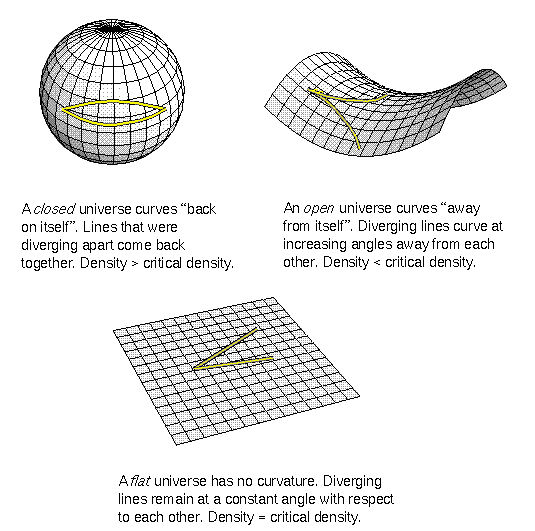
\includegraphics[scale=0.5]{images/universefate (1).png}
    \caption{The Three Fates of the Universe}
    \label{fig:universalfate}
\end{figure}
\FloatBarrier
Which state our universe will head towards depends on a quantity called the critical density $\rho_{crit}$,
\begin{equation}\label{eq:rhocrit1}
    \rho_{crit} = \frac{3 H_0 ^2}{8 \pi G}
\end{equation}
Where $H_0 = 65 \: Mpc \: km/s $ is the Hubble constant and $G = 6.67 \times 10^{-11} \: N m^2 / kg^2$ is the universal gravitation constant. Density is generally mass divided by volume, and substituting constants into (\ref{eq:rhocrit1}) after conversion yields:

\begin{equation}\label{eq:rhocrit2}
    \rho_{crit} \approx 10^{-26}  \: kg/m^3
\end{equation}
Which is extremely tiny, roughly 5 hydrogen atoms per cubic meter. This critical density is roughly equivalent to the density of the Milky Way \cite{Impey2023}. Currently, the flat universe candidate is the most probable, but I do not have complete data on the composite mass of the universe due to difficulties in detecting dark matter. Being able to calculate it could provide insight into this question, making it highly relevant in the modern astrophysics community. This essay will apply the viral theorem approach to the Fornax and Virgo cluster candidates, employing various concepts like Newtonian gravitation and field potentials. Synthesis of experimental data collected from the McDonald's observatory and astronomical surveys published online will be used. By computing the total mass generated from the virial theorem, I will compare it to measured mass-luminosity ratios and attribute the difference to dark matter, as it will not contribute to luminosity.

\section{Galactic Clusters and Dark Matter}
In ancient times, Earth was thought to be the center of the universe in the geocentric model, put forward by Claudius Ptolemy. This model led to the emergence of the celestial sphere, an imaginary sphere projected above the earth's surface which acts as a template for various coordinates and celestial markers.. On this imaginary sphere, the North and South Celestial Poles corresponded with Earth's geographic poles. The celestial equator was derived from Earth’s equator, serving as a reference plane to facilitate the positioning of stars and planets.\\
Describing the position of these planets and galaxies uses two celestial coordinates: right ascension and declination. Right ascension measures the angular distance between a celestial object and the vernal equinox, using time units—hours, minutes, and seconds. This measurement mode finds its rationale in the Earth's rotation, where roughly every hour of right ascension corresponds to a 15-degree shift. Declination can be seen as an evolution of latitude measurements, projected onto the celestial sphere, indicating the angular position of a star above or below the celestial equator.\\
Aside from describing the position of galaxies, there are two other quantities associated with their motion: radial velocity and tangential velocity. Recessional Velocity can be directly calculated from the measured redshift due to the Doppler effect, indicating the speed at which an object moves towards or away from the observer. Tangential velocity, on the other hand, is the movement of galaxies perpendicular to the line of sight and is discerned by tracking the object against a relatively stationary background over prolonged periods. These can be described through vector properties: the overall velocity of a body is equivalent to the vector addition of tangential and recessional velocities.\\
Discussing clusters themselves, galactic clusters are structures that consist of hundreds to hundreds of thousands of galaxies that are bound in proximity by the gravitational force. Generally, these galaxies travel with a recessional velocity within the cluster around some center-of-mass point. In the astronomical community, it is generally agreed upon that most galactic clusters contain roughly 85\% dark matter and 15\% visible matter. As a result, it is mostly dark matter that binds the galaxies together \cite{DarkMatter}.  
\subsection{Relating Force to Potential Energy}
The two significant types of forces being discussed are conservative and non-conservative forces. Conservative forces perform the same amount of work despite different trajectories; they only depend on displacement. Non-conservative forces, on the other hand, depend on the path taken and when computing the work done by them. The gravitational force field is a conservative force, while frictional forces are non-conservative. Conservative forces have a unique property that
\begin{equation}\label{eq: force-nablaU}
    \vec{F} = -\nabla U
\end{equation}
Where $\vec{F}$ is the force vector and $U$ is the potential energy as a function of position. The $\nabla$ operator is a transformation that, in Cartesian coordinates, creates a directional vector with $n$ components using the partial derivative in $n$ dimensions:
\begin{equation} \label{eq:nabladefinition}
\nabla f(x,y,z, ..., n) = \begin{pmatrix}
    \frac{\partial f}{\partial x} \\
    \frac{\partial f}{\partial y} \\
    \frac{\partial f}{\partial z} \\
    \vdots\\
    \frac{\partial f}{\partial n} \\
\end{pmatrix}
\end{equation}

The partial derivative is identically computed to a derivative with the exception that every variable outside of the one being differentiated with respect to is treated as a constant. This property allows the $\nabla$ operator to create a gradient vector for its scalar function, one that defines the direction of its slope field at any given point. This can be applied to compute the gravitational potential energy in the case of a galactic cluster, where I first approximate the force using Newton's law of universal gravitation. Let us define the total mass $M$ of a galactic cluster equal to $Nm$, where $N$ is the number of galaxies and $m$ is their average mass. Substituting this into Newton's Law of Universal Gravitation:
\begin{equation}
    F = -\frac{GM^2}{R^2}
\end{equation}
Where $R$ is the radius of the cluster, assuming it is spherical. This means that the gradient only takes into account one variable, the radial distance $r$, so the partial differentiation is identical to regular differentiation with respect to r. Substituting this expression (in a general form with $r$ instead of $R$ into (\ref{eq: force-nablaU}):

$$
    \vec{F} = -\frac{\partial U}{\partial r} \Rightarrow -\int \vec{F} \cdot \: d\vec{r} = \vec{dU}
$$
Computing the integral to find an expression for $U(r)$:
\begin{equation}\label{eq:potentialenergy}
    -\int - (-\frac{GM^2}{r^2})\: dr = - \frac{GM^2}{r} = U(r)
\end{equation}
Hence the equation for the gravitational potential energy of the total cluster is simply
$$ U = -\frac{GM^2}{R}$$

\section{The virial theorem}
Using the virial theorem, and assuming $\vec{F_k}$ is a  conservative force, one can substitute $-\nabla U_k$ for $\vec{F_k}$. When summing all of the particles, this gradient simplifies into the total 
$$\langle T \rangle = -\frac{1}{2}  \sum_{k=1}^{N} \langle \nabla U_k \cdot \vec{r_k} \rangle = -\frac{1}{2} 
 \langle -\nabla U \cdot \vec{r} \rangle $$ 
My expression for gravitational potential energy is spherically symmetric. In spherical symmetry, the only component that changes is the radial distance from the center of the particle arrangement, so the gradient transforms into a partial derivative with respect to $r$.
$$
  \langle T \rangle = \frac{1}{2} \langle \nabla U \cdot \vec{r} \rangle  \\
  = \frac{1}{2} \langle r\frac{\partial{U}}{\partial{r}} \rangle
$$
The dot product of two vectors is defined as
\begin{equation} \label{eq: dotproduct}
    \textbf{a} \cdot \textbf{b} = \abs{\textbf{a}} \abs{\textbf{b}} \cos{\theta}
\end{equation}
The dot product of $\vec{r}$ and $\frac{\partial U}{\partial r}$ was simplified to multiplying the magnitude of the position vector $\vec{r}$ with the magnitude of the gradient vector because they are both parallel ($\theta = 0^o$, so $\cos{\theta} = 1$), as illustrated in \textbf{Figure \ref{fig:gradientparalleltorl}}.
\begin{figure}[h!]
    \centering
\begin{tikzpicture}[scale=1.5, >=Stealth]
  % Define the center of the potential field
  \coordinate (O) at (0,0);
  
  % Draw the particle at some position
  \coordinate (P) at (2,0);
  \fill (P) circle (2pt) node[above right] {Particle};
  
  % Draw the position vector
  \draw[->, thick] (O) -- (1.9,0) node[midway, below] {$\mathbf{r}$};
  
  % Draw the gradient vector
  \draw[->, thick, red] (O) -- ++(1.3,0) node[above] {$\frac{\partial U}{\partial r}$};
  
  % Draw the center
  \fill (O) circle (1pt);
  
  % Draw the gravitational potential field (arrows)
  \foreach \angle in {0,10,...,360} {
    \draw[->, dashed, blue!50] (O) -- (\angle:1.8cm);
  }
  
  % Optionally, draw a dashed circle to represent the equipotential
  \draw[dashed, blue] (O) circle (2cm);
    \draw[dashed, blue] (O) circle (1.2cm);
      \draw[dashed, blue] (O) circle (0.5cm);
  
  % Label the angle, which is 0 in this case
  % Since the angle is 0, the label is not necessary but can be included for completeness
  % \draw (0.5,0) arc (0:0:0.5cm) node[right] {$\theta = 0^\circ$};
\end{tikzpicture}
    \caption{A Particle Within a Radial Potential Field}
    \label{fig:gradientparalleltorl}
\end{figure}


Substituting the derived expression for gravitational potential energy $U$ in equation \ref{eq:potentialenergy}:
$$ r \frac{\partial U}{\partial r} = r \: \frac{\partial}{\partial r} (\frac{GM^2}{r}) = (-1)(r) \frac{-GM^2}{r^2}$$
Substituting this into the expression for the mean of the total kinetic energy of the particles $\langle T \rangle$:
$$ \langle T \rangle = (\frac{1}{2}) \langle \frac{GM^2}{r} \rangle = \frac{1}{2} \langle U \rangle $$ 
The mean of the total kinetic energy is expressed in terms of the potential energy of a spherical cluster. Using the definition of the mean kinetic energy $\langle T \rangle$, given by
\begin{equation}\label{eq:avgkineticenergy}
   \langle T \rangle  = \frac{1}{2} M \langle v \rangle ^2 = \frac{1}{2} \langle U \rangle
\end{equation}
Where $\langle v \rangle$ is the mean recessional velocity of the particles within the cluster, it is evident that the mean kinetic energy is equal to the mean potential energy. Galaxies within a cluster have been observed to have a mostly uniform recessional velocity, and taking the mean of their recessional velocities and multiplying it with the total mass of the cluster is approximately equal to finding the kinetic energy of each galaxy individually and then summing this over the total number of galaxies, which each have distinct recessional velocities and masses. This method is preferred as, in the context of astrophysics, the fractional uncertainty is extremely small, and it is much more convenient than summing each galaxy because some clusters have upwards of 1000 galaxies -many of which do not have reliable data regarding their recessional velocities. To clarify, all uncertainty is calculated by dividing the range of values by two for data sets, and otherwise, is the instrumental uncertainty. Substituting the expression for $U$ that was previously determined into equation \ref{eq:avgkineticenergy}:
$$ U = \frac{GM^2}{2R} = \frac{1}{2}M \langle v \rangle ^2$$
Rearranging to solve for the total mass $M$

\begin{equation} \label{eq:massofcluster}
    M \approx \frac{R \langle v \rangle^2}{G} 
\end{equation} 

This approximation for the mass of a galactic cluster assumes the cluster is spherical. From this assumption, it is also assumed that the radius of the galactic cluster is a constant and that the only significant gravitational forces acting on the galaxies within the cluster are contributed to by other galaxies within the cluster -no extraneous mass is affecting this cluster significantly. While this model is derived assuming a colloidal suspension of particles as the context, at the scale of clusters, galaxies can be viewed as particles suspended together by the gravitational force, thus allowing a valid approximation for the mass of a cluster. There are relativistic approximations for cluster mass that are precise for ellipsoid clusters and other various shapes, but they demand data inaccessible to a typical student and contain mathematics well beyond this scope\cite{libretexts}. (\ref{eq:massofcluster}) proposes two quantities that must be experimentally determined: the mean recessional velocity of the galaxies within the cluster and the radius of the cluster.

\subsection{Methodology}
For the two unknown values, the radius of the galactic cluster and mean recessional velocity, the following methodology will compute them for both clusters. The recessional velocity will be determined experimentally by measuring redshift, and other values that cannot be determined with the available resources will be collected from online sources that will be discussed shortly. Redshift $z$ is related to the recessional velocity $v_r$ by the following equation:
\begin{equation}\label{eq:redshift}
    z = \frac{\Delta \lambda}{\lambda_{obs}} = \frac{v_r}{c}
\end{equation}
Where $c$ is the speed of light, $2.998 \cdot 10^8 \: m/s$, and $\Delta \lambda$ is the difference between observed and actual wavelength. The actual wavelengths will be found online, particularly in TheSkyLive and SINBAD, while observed wavelengths will be measured directly using a spectrometer\cite{TheSky}. Because recessional velocity is relatively homogeneous for galaxies within the same clusters, it will be used as the defining variable for removing outliers from data sets. To determine the radius, the range of right ascension values will be used to find an angle, which can then be multiplied by the cluster's distance to compute the diameter. Dividing this by two and combining it with the value for the mean recessional velocity will allow for the calculation of the total mass of the cluster. Then, based on the measured luminosity of the cluster, the mass-luminosity ratio of the cluster can be compared to the mass-luminosity ratio of the constituent galaxies found through outdated methods of direct observation in the aforementioned databases, and the difference can be attributed to dark matter. This is possible because the methods used by astronomers to determine the mass-luminosity ratios in previous iterations of the databases were not ones that accounted for Dark Matter, though they are not detailed on the sites. As a result, it is expected that the computed mass-luminosity ratio will be much greater than the established ones, and a comparison between both ratios is effective since both galaxies and clusters are thought to be made up of about 85\% Dark Matter.
\section{Experimental Data}
The Fornax and Virgo clusters were chosen as candidates for this method due to the extensive studies with them as subjects and reliable data to be synthesized with experimentally determined data. For galaxies that were not visible nor present in the ACS survey, NED, TheSkyLive, and SIMBAD databases were used to generate the table of viable candidates below\cite{SIMBAD}\cite{NGC}\cite{TheSky}\cite{ACSVCS_Publications_2024}:

\subsection{Galaxy Data}

\begin{table}[!htp]
    \centering
    \caption{Galactic Data: Virgo and Fornax Clusters}
    \label{tab:galactic_data}
    \begin{minipage}[t]{.45\linewidth}
        \centering
        \scriptsize
        \begin{tabular}{lrrrr}
            \toprule
                Name & RA (h m s) & Dec (° ' '') & Mag & RV (km/s) \\
                    \midrule
VCC 1226 &12 29 46.79 &08 00 01.5 &9.31 &997 \\
VCC 1316 &12 30 49.42 &12 23 28 &9.58 &1307 \\
VCC 1978 &12 43 39.66 &11 33 09.4 &9.81 &1117 \\
VCC 881 &12 26 11.74 &12 56 46.4 &10.06 &-244 \\
VCC 798 &12 25 24.04 &18 11 25.9 &10.09 &729 \\
VCC 763 &12 25 03.72 &12 53 13.2 &10.26 &1060 \\
VCC 731 &12 24 28.20 &07 19 03 &10.51 &1243 \\
VCC 1535* &12 34 03.10 &7 41 59 &10.61 &448 \\
VCC 1903 &12 42 02.4 &11 38 48 &10.76 &410 \\
VCC 1632 &12 35 39.82 &12 33 22.6 &10.78 &340 \\
VCC 1231* &12 29 48.87 &13 25 45.7 &11.1 &2244 \\
VCC 2095 &12 52 56.00 &11 13 53 &11.18 &984 \\
VCC 1154 &12 29 00.03 &13 58 42.9 &11.37 &1210 \\
VCC 1062* &12 28 03.90 &09 47 14.0 &11.4 &532 \\
VCC 2092 &12 52 17.50 &11 18 50.0 &11.51 &1377 \\
VCC 369 &12 19 45.42 &12 47 54.3 &11.8 &1009 \\
VCC 759 &12 24 55.50 &11 42 15.0 &11.8 &943 \\
VCC 1692 &12 36 53.40 &07 14 47.0 &11.82 &1730 \\
VCC 1030 &12 27 40.49 &8 14 47.0 &11.84 &801 \\
VCC 2000 &12 44 31.95 &11 11 25.1 &11.94 &1083 \\
VCC 685 &12 23 57.90 &16 41 37.0 &11.99 &1241 \\
VCC 1664* &12 36 26.86 &11 26 20.6 &12.02 &1142 \\
VCC 654 &12 23 35.28 &16 43 22.3 &12.03 &950 \\
VCC 944* &12 26 50.53 &09 35 02.0 &12.08 &843 \\
VCC 1938 &12 42 47.40 &11 26 33.0 &12.11 &1164 \\
VCC 1279* &12 30 17.39 &12 19 43.9 &12.15 &1349 \\
VCC 1720 &12 37 30.61 &09 33 18.8 &12.29 &2273 \\
VCC 355 &12 19 30.61 &14 52 41.4 &12.41 &1359 \\
VCC 1619 &12 35 30.61 &12 13 15.4 &12.5 &381 \\
VCC 1883 &12 41 32.70 &07 18 53.0 &12.57 &1875 \\
VCC 1242 &12 29 53.49 &14 04 07.0 &12.6 &1609 \\
VCC 784 &12 25 14.75 &15 36 27.2 &12.67 &1069 \\
VCC 1537 &12 34 06.10 &11 19 17.0 &12.7 &1374 \\
VCC 778 &12 25 12.27 &14 45 43.8 &12.72 &1375 \\
VCC 1321 &12 30 52.21 &16 45 32.6 &12.84 &967 \\
VCC 828 &12 25 41.70 &12 48 38.0 &12.84 &561 \\
VCC 1250 &12 29 59.10 &12 20 55.0 &12.91 &1970 \\
VCC 1630 &12 35 37.97 &12 15 50.5 &12.91 &1172 \\
VCC 1146 &12 28 57.56 &13 14 30.8 &12.93 &635 \\
VCC 1025* &12 27 36.71 &08 09 14.8 &13.06 &1071 \\
VCC 1303 &12 30 40.64 &09 00 55.9 &13.1 &875 \\
VCC 1913 & 12 42 10.70 &07 40 37.0 &13.22 &1892 \\
VCC 1327 & 12 30 57.56 &12 16 17.2 &13.26 &150 \\
VCC 1125 &12 28 43.37 &11 45 21.0 &13.3 &195 \\
VCC 1475* & 12 33 04.95 &16 15 55.9 &13.36 &951 \\
VCC 1178 &12 29 21.30 &08 09 23.0 &13.37 &1243 \\
VCC 1283 & 12 30 18.40 &13 34 40.9 &13.45 &876 \\
VCC 1261 &12 30 10.39 &10 46 46.1 &13.56 &1871 \\
VCC 698 & 12 24 05.00 &11 13 06.0 &13.6 &2080 \\
VCC 1422 & 12 32 14.21 &10 15 05.0 &13.64 &1288 \\
VCC 2048 &12 47 15.32 &10 12 13.0 &13.81 &1084 \\
VCC 1871 & 12 41 15.72 &11 23 13.5 &13.86 &567 \\
VCC 9 & 12 09 22.34 &13 59 33.1 &13.93 &1804 \\
VCC 575 & 12 22 43.31 &08 11 53.7 &14.14 &1231 \\
VCC 212 &12 43 15.32 &08 10 53.4 &13.11 &1881 \\
 \bottomrule
        \end{tabular}
         \caption*{Virgo Data}
    \end{minipage}\hfill
 \begin{minipage}[t]{.45\linewidth}
        \centering
        \scriptsize
        \begin{tabular}{lrrrr}
            \toprule
            Galaxy & RA (h m s) & Dec (° ' '') & Mag & RV (km/s) \\
            \midrule
FCC 21* &03 22 42.09 &-37 12 31.63 &9.4 &1760 \\
FCC 213 &03 38 29.14 &-35 27 02.30 &10.6 &1425 \\
FCC 219 &03 38 52.08 &-35 35 37.67 &10.9 &1947 \\
NGC 1340 &03 28 19.7 &-31 04 05 &11.3 &1169 \\
FCC 167 &03 36 27.45 &-34 58 31.09 &11.3 &1877 \\
FCC 276 &03 42 19.16 &-35 23 36.03 &11.8 &1388 \\
FCC 147 &03 35 16.74 &-35 13 33.94 &11.9 &1294 \\
IC 2006 &03 54 28.45 &-35 58 01.7 &12.2 &1382 \\
FCC 83 &03 30 35.04 &-34 51 14.51 &12.3 &1514 \\
FCC 184 &03 36 56.84 &-35 30 23.85 &12.3 &1302 \\
FCC 63 &03 28 06.55 &-32 17 43.35 &12.7 &1392 \\
FCC 193 &03 37 11.67 &-35 44 39.73 &12.8 &921 \\
FCC 170 &03 36 31.59 &-35 17 43.34 &13 &1724 \\
FCC 153 &03 35 30.91 &-34 26 44.74 &13 &1619 \\
FCC 177 &03 36 47.35 &-34 44 17.25 &13.2 &1561 \\
FCC 47 &03 26 31.97 &-35 42 44.59 &13.3 &1418 \\
FCC 43 &03 26 02.30 &-32 54 36.80 &13.5 &1323 \\
FCC 190 &03 37 08.86 &-35 11 37.54 &13.5 &1740 \\
FCC 310 &03 46 13.67 &-36 41 43.24 & 12.1 &1373 \\
FCC 249 &03 40 41.92 &-37 30 33.30 &13.6 &1613 \\
FCC 148 &03 35 16.79 &-35 15 55.95 &13.6 &740 \\
FCC 255 &03 41 03.40 &-33 46 38.42 &13.7 &1255 \\
FCC 277* &03 42 22.60 &-35 09 10.22 &13.8 &1640 \\
FCC 55* &03 27 17.90 &-34 31 29.17 &13.9 &1279 \\
FCC 152 &03 35 33.09 &-32 27 44.79 &14.1 &1380 \\
FCC 301 &03 45 03.49 &-35 58 16.95 &14.2 &1007 \\
FCC 335 &03 50 36.64 &-35 54 29.27 &14.2 &1430 \\
FCC 143 &03 34 59.06 &-35 10 09.90 &14.3 &1334 \\
FCC 95 &03 31 24.68 &-35 19 46.41 &14.6 &1275 \\
FCC 136 &03 34 29.39 &-35 32 41.18 &14.8 &1205 \\
FCC 182 &03 36 54.24 &-35 22 22.69 &14.9 &1657 \\
FCC 204 &03 38 13.60 &-33 07 31.29 &14.9 &1369 \\
FCC 119 &03 33 33.73 &-33 34 17.84 &15 &1374 \\
FCC 90 &03 31 09.06 &-36 17 19.47 &15 &1813 \\
FCC 26 &03 23 37.16 &-35 46 38.68 &15 &1823 \\
FCC 106 &03 32 47.62 &-34 14 14.18 &15.1 &2064 \\
FCC 19* &03 22 22.77 &-37 23 45.55 &15.2 &1497 \\
FCC 202 &03 38 06.40 &-35 26 17.96 &15.3 &808 \\
FCC 324* &03 47 52.61 &-36 28 13.25 &15.3 &1856 \\
FCC 288* &03 43 22.61 &-33 56 14.78 &15.4 &1189 \\
FCC 303 &03 45 13.93 &-36 56 07.63 &15.5 &1980 \\
FCC 203* &03 38 09.10 &-34 31 01.08 &15.5 &1138 \\
NGC 854 &02 11 30 &-35° 50’ 06” & &6148 \\
NGC 1217* &03 06 06 &-39 02 11 & & 6196 \\
IC 1862 &02 51 59 &-33 20 25 & &6423 \\
      \bottomrule
        \end{tabular}
        \caption*{Fornax Data}
    \end{minipage}
\end{table}

The data in \textbf{Table \ref{tab:galactic_data}} does not make use of a comprehensive list of all possible galaxies in the Fornax / Virgo clusters, but one of all that are highly likely to be in Fornax based on cross-reference - only galaxies that were present on all databases with recessional velocity (RV) values within 10\% of each other were considered. Galaxies that were present on all databases but had significantly varying RV values were then observed experimentally, and asterisks mark these entries. Using equation \ref{eq:redshift}, the recessional velocity was computed for these data points, and other values can be directly measured. The measured observed redshifts are tabulated in \textbf{Ap.4} for Virgo and \textbf{Ap.5} for Fornax, which was cross-referenced online from a survey taken in 2021 for Fornax that observed 8 of the galaxies \cite{FornaxArticle}. For Virgo, little data was available online, so whatever data was calculated experimentally was used, and these points fell close to the average with the exception of the entry for NGC 1217, which had a very high recessional velocity similar to some other outliers. It is likely that these galaxies (NGC 1217, 854, and IC 1862) are near the cluster and bound gravitationally, as their RA and Dec are somewhat similar.\\
This synthesis of data was necessary because the ACS survey, which sourced many of the galaxies, was outdated, containing galaxies that are now evidently not part of the cluster due to massive discrepancies in recessional velocities. While an ACS survey is normally considered to be reliable and concrete, this particular survey was created over 30 years ago. Therefore, this data is somewhat unreliable, but the large amount of entries makes the mean less altered by these discrepancies. For example, take the last few entries in the table, all of which have incredibly high recessional velocities. As discussed before, most galaxies in a cluster have somewhat uniform recessional velocities, so this is very obviously indicative of galaxies that either belong to another cluster or are free-floating / unbound. The left-hand side table corresponds to data gathered for the Virgo Cluster and the right-hand side for the Fornax Cluster\cite{Jordan2004SurveyII}\cite{Cote2004SurveyI}\cite{Mei2005SurveyV}.


\FloatBarrier
\section{Data Analysis}
For the Fornax cluster, the groupings of galaxies were concentrated around the 800-1600 km/s recessional velocity range. 
\begin{figure}[h!]
    \centering
    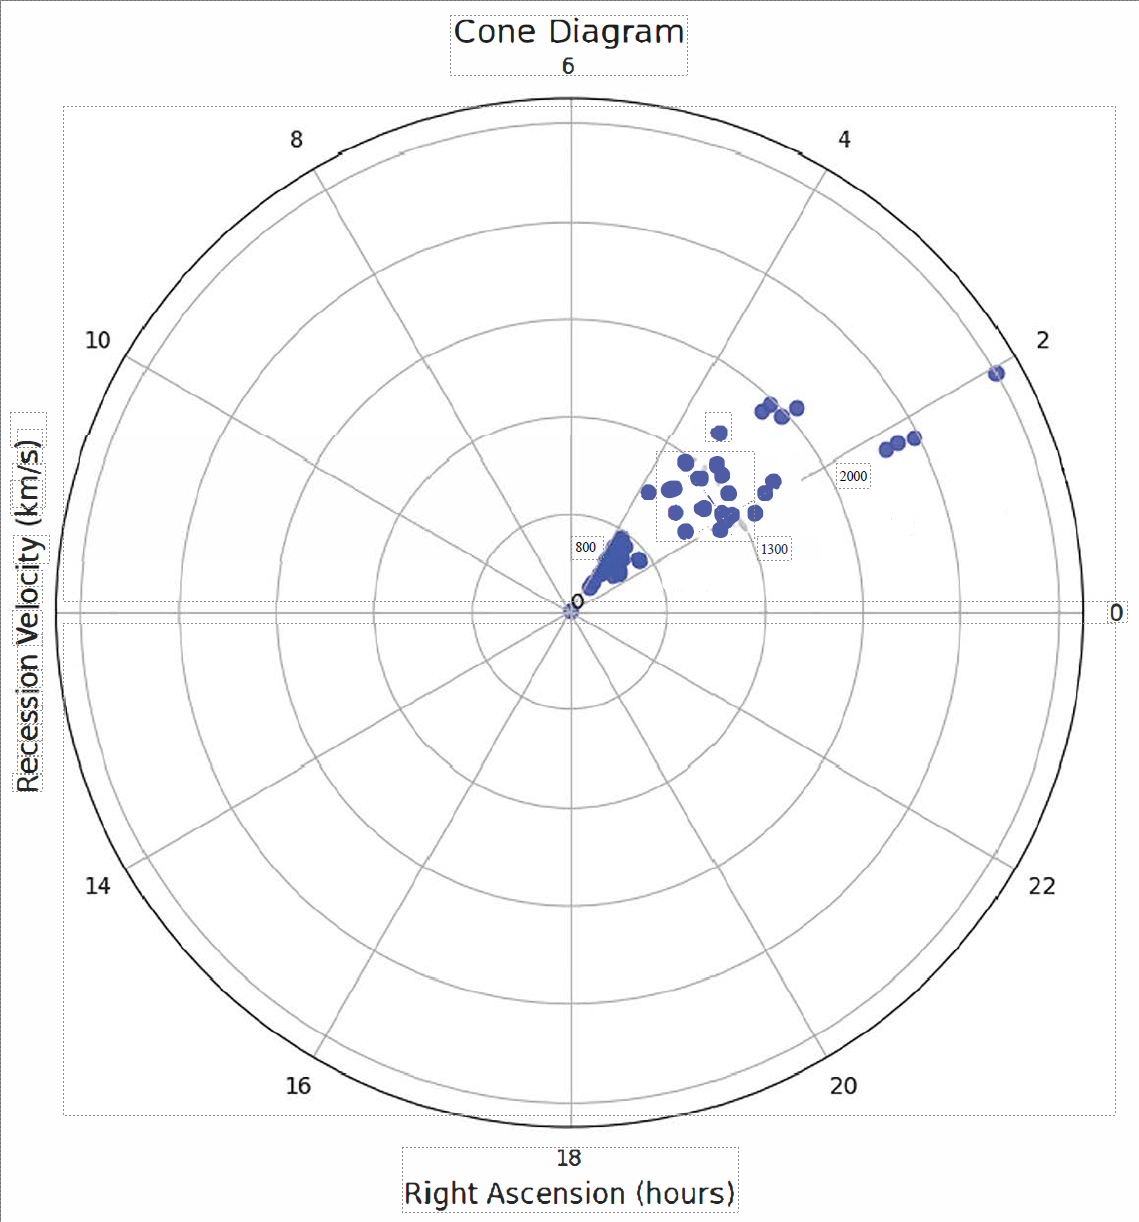
\includegraphics[scale=0.5]{images/output_0_0.png}
    \caption{A polar plot of the Fornax cluster's recession velocity vs right ascension}
    \label{fig:polarfornax}
\end{figure}
    
After gathering this data, the code in (\textbf{Ap.2}) was created to remove all data values that were $\pm 3\sigma $ from the mean of the data set (a convention in astronomy). The remaining valid data points were then used to calculate the mean velocity of the galaxies using the Python code in \textbf{Ap.3}. Hence, $\langle v \rangle $ has been computed for the Fornax cluster:
$$ \langle v \rangle = 1783 \pm 662 \: km/s$$
The Virgo cluster used a similar set of code and the same methodology, simply with differing data points, shown in \textbf{Ap.3}, providing:
$$ \langle v \rangle = 1061 \pm 1244 \, km/s$$
\subsection{Further Data Collection}
From these validated data points, the distance of some galaxies was experimentally determined by observing the parallax angle
\begin{equation}
    d_{ps} = \frac{1}{p''}
\end{equation}
The process is as follows: the telescope tracks the image of the galaxy as it moves across the sky and one time period and compares its position at another time period over the course of 6 months. After doing this, the angle it has traveled is the measured parallax angle, and its reciprocal gives the star's distance in parsecs. The galaxies whose distance I could not find online for the Fornax and Virgo clusters were observed for a period of time using a refractor telescope in the McDonald's Observatory, and parallax angles were measured for almost all of them. There were relatively few galaxies that had no data, and the following averages were collected: $(5.46448 \pm 0.64538)\cdot 10^{-8}$ for Fornax and $(6.329 \pm 0.896 ) \cdot 10^{-8} $ for Virgo\cite{Mei2005SurveyIV}. The raw experimental data is in \textbf{Ap.6,7} for Virgo and Fornax respectively, and this was synthesized with the values I found on the aforementioned databases. 
\FloatBarrier

\begin{figure}[h!]
    \centering
    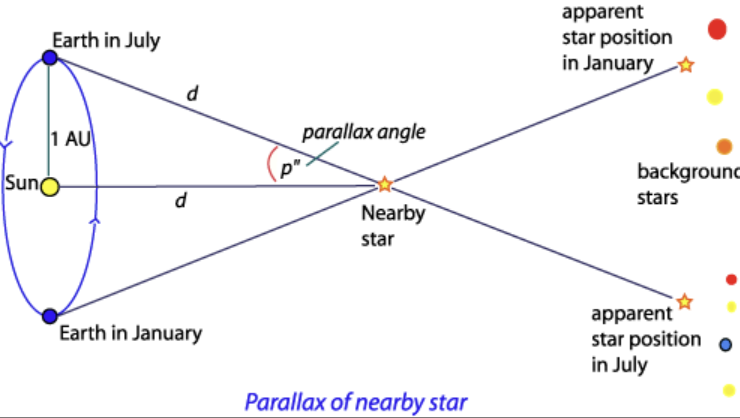
\includegraphics[scale=0.6]{images/parallax.png}
    \caption{Parallax Angle Measurement Process}
    \label{fig:parallax}
\end{figure}

\FloatBarrier
Alongside this, the absolute luminosities were measured to be about $(5.55 \pm 0.01) \cdot 10^{11} \: L\textsubscript{\(\odot\)}$ for Virgo and $ (17.8 \pm 0.1 ) \cdot 10^{11} \: L\textsubscript{\(\odot\)}$ for Fornax. L\textsubscript{\(\odot\)} is solar luminosity, which is equal to the sun's luminosity $3.846 \times 10^{26}$ \cite{sunluminosity}.

\FloatBarrier
\section{Applying Data  to the Model}
Now that the mean recessional velocity has been determined for both clusters, the radius must be determined. Visualizing either the Fornax or Virgo cluster below, it becomes apparent that the combed data set (represented by the point within the boundary) contains maximum and minimum points that can be used to compute the radius. Using the identity that $s= r\theta$, where $\theta$ is the range of right ascension values converted to degrees. This range will yield a diameter of $2R$. The distance, or $r$ in the equation, can be computed by finding the average of the furthest and closest distances measured through the parallax angle observations. This continues to rely heavily on the sphere approximation and assumes that the vertical distribution of galaxies across the two-dimensional projection is somewhat similar to the right ascension distribution. The more different they are, the less accurate this answer will be.
\FloatBarrier
\begin{figure}[h!]
    \centering
\begin{tikzpicture}[scale=0.7]
%		%Grid
%		\draw[thin, dotted] (0,0) grid (8,8);
%		\foreach \i in {1,...,8}
%		{
%			\node at (\i,-2ex) {\i};	
%		}
%		\foreach \i in {1,...,8}
%		{
%			\node at (-2ex,\i) {\i};	
%		}
%		\node at (-2ex,-2ex) {0};
		
		% Coordinates
		\node[mass] (O) at (0,0) {};
		\coordinate (A) at (3.5,3);
		\coordinate (B) at (5.5,2.5);
		\coordinate (C) at (7.3,4);
		\coordinate (D) at (6.5,5.5);
		\coordinate (E) at (4,6);
		\coordinate (F) at (2.5,4);
		\node[mass] (G) at (3.2,5.8) {};
		\node[mass] (H) at (6.6,3.3) {};
		%% Nodes
%		\foreach \i in {A,B,...,F}
%		{
%			\node at (\i) {\i};
%		}
		
		
		% Body
		\draw[thick] (A) to[out=-60, in=200, looseness=1.5] (B) to[out=10, in=220, looseness=1.5] (C) to[out=40, in=-60, looseness=1] (D) to[out=120, in=-10, looseness=1] (E) to[out=170, in=60, looseness=1.5] (F) to[out=240, in=140, looseness=1.5] cycle;
		
		% Masses
		% In the Body
		\foreach \i in {1,2,...,10}
		{
			\pgfmathsetmacro{\xcoor}{2*rand + 5} % x-coordinate
			\pgfmathsetmacro{\ycoor}{1.5*rand + 4} % y-coordiante 
				
			\draw[fill=black] (\xcoor, \ycoor) circle (0.8pt);
		}
		% Out of the Body
		\foreach \i in {1,2,...,10x0}
		{
			\pgfmathsetmacro{\xcoor}{2.7*rand + 5} % x-coordinate
			\pgfmathsetmacro{\ycoor}{2.4*rand + 4} % y-coordiante 
				
			\draw[fill=black] (\xcoor, \ycoor) circle (0.8pt);
	}
		\draw[fill=black] (G) circle (0.8pt);
		\draw[fill=black] (H) circle (0.8pt);
		
		% Nodes
		\node (s) at (3,7) {Cluster Boundary};
        \node at (5,5) {2R};
		
		% Lines
		\draw[-latex] (O) -- (G) node [pos=0.5, above left] {$RA_{min}$};
		\draw[-latex, blue] (G) -- (H) node [pos=0.6, above left] {$\vb*{}$};
		\draw[-latex] (O) -- (H) node [pos=0.5, below right] {$RA_{max}$};
		\draw[-latex] (s) to[bend right=50] (3,5.8);
		
		% Point
		\draw[fill=black] (O) circle (1pt) node [below, shift={(0,-0.1)}] {$\mathrm{O}$};
	\end{tikzpicture}
    \caption{Visualization of the Radius Approximation}
    \label{fig:enter-label}
\end{figure}
\FloatBarrier
Using the same code from the previous section, the following values were found for the Fornax and Virgo cluster's right ascension ranges in degrees, noting that 15 degrees correspond to one hour of RA. For Fornax, $58.167^o$ was the max, and $49.5151^o$ was the minimum. Therefore, the value of $\theta$ is $(8.652 \pm 4.326)^o$. For Virgo, $192.87^o$ was the maximum RA, and $184.32^o$ was the minimum. Therefore, $\theta$ is $( 8.55\pm 4.28)^o$. The ranges and averages of the maximum and minimum parallax angles of galaxies within each cluster were determined similarly from the previous section. Taking the reciprocal of the angles gives $(18.8790 \pm 2.3002) \cdot 10^{6}$ parsecs for Fornax and $(15.89 \pm 2.26)\cdot 10^6$ parsecs for Virgo. This equals $(58.2545 \pm 7.0978 )\cdot 10^{19} \:km$ for Fornax and $ (49.03 \pm 6.98)\cdot 10^{19}\:km$ for Virgo. Computing their respective radii
$$ R_{Fornax} = \frac{r \theta}{2} \Rightarrow \frac{1}{2}((58.2545 \pm 7.0978 )\cdot 10^{19})(8.652 \pm 4.326) = (2.52 \pm 1.30) \cdot 10^{21}\:km$$
$$ R_{Virgo} = \frac{r \theta}{2} \Rightarrow \frac{1}{2}((49.03 \pm 6.98)\cdot 10^{19})( 8.55 ± 4.28) = (2.10 \pm 1.09 )\cdot 10^{21}\:km$$
Substituting this into (\ref{eq:massofcluster}) I find that:
$$ M_{Fornax} = \frac{\langle v \rangle ^2 R}{G} \Rightarrow \frac{((1783 \pm 662) \cdot 10^3)^2 ((2.52 \pm 1.30) \cdot 10^{21})}{G} = (1.20 \pm 1.09) \cdot 10^{44} \: kg$$
$$ M_{Virgo} =  \frac{\langle v \rangle ^2 R}{G} \Rightarrow \frac{((1061 \pm 1244)\cdot 10^3)^2 ((2.10 \pm 1.09) \cdot 10^{21})}{G} = (3.54 \pm 8.51 ) \cdot 10^{43} \: kg$$
Converting to solar masses ($M\textsubscript{\(\odot\)}$), I find
$$M_{Fornax} = (6.04 \pm 5.46) \cdot 10^{13} M_\textsubscript{\(\odot\)} \hspace{15pt} M_{Virgo} = (1.78 \pm 4.28))\cdot 10^{13} M_\textsubscript{\(\odot\)} $$
I can then compute the mass-luminosity ratios of either cluster.
$$M/L _{Fornax} = (108.83 \pm 98.38) \frac{M_\textsubscript{\(\odot\)}}{L_\textsubscript{\(\odot\)}} \hspace{15pt} M/L_{Virgo} = (10.00 \pm 24.05) \frac{M_\textsubscript{\(\odot\)}}{L_\textsubscript{\(\odot\)}}$$
Comparing these with the average mass-luminosity ratios of the galaxies of each cluster, which were established in astronomical literature to generally be about 15.53 for Fornax and 0.9 for Virgo, it is found that\cite{lindblad}:
$$(1-\frac{15.53}{108.8}) \cdot 100\% = 85.7\% = \text{Dark Matter Concentration of Fornax}$$
$$ (1-\frac{0.9}{10.0}) \cdot 100\% = 91.1\% = \text{Dark Matter Concentration of Virgo} $$
The mean values excluding uncertainty were used for this and parts of the following analysis because the uncertainties are too large to draw significant conclusions.
\FloatBarrier
\section{Evaluation}
\noindent The cross-verification of data collected for NED and SIMBAD with the ACS survey and McDonald's laboratory observations made most of the data reliable and accurate. The percentage uncertainty for the mean recessional velocities of the Fornax and Virgo clusters were about 90.4\% and 240.5\%, respectively, so there very clearly were sources of error throughout the methodology.\\
\noindent The largest source of error arises from the spherical approximation, as the Virgo cluster deviated significantly further from the 85\% estimated dark matter concentration than the Fornax cluster. Another source of error could have been the approximated average distance of the cluster using the parallax angle. \\
\noindent Furthermore, using parallax angles found both online and experimentally to find the distance, while convenient, could be made more accurate by using tertiary distance indicators as an alternative method. However, utilizing this is more difficult to access experimentally and would likely have to be found online by published sources. Another source of inaccuracy is the type of telescope used for the apparent magnitude measurements, which was a refractor telescope with a significantly smaller lens than others, though not available to non-faculty members. Refractor telescopes contain an objective lens in front of the eyepiece lens, and the larger the area of the objective lens, the more light-gathering power (LGP) it has (see \textbf{Ap.1})\cite{Impey2023}:
\begin{equation}
    LGP = 4\pi D^2
\end{equation}
\noindent Where $D$ is the diameter of the objective, the refractor telescope used for the Virgo cluster was also a different telescope - despite having the same specifications and being an identical model, it was a few years older. Refractor telescopes require constant maintenance of glass, so this could have contributed to further deviation for the Virgo cluster outside of its less spherical shape.\\
\noindent It can also be questioned how applicable this model is across various astronomical objects. Generally speaking, clusters with galaxies with a range in distances closer to the estimated radius from the range in right ascension values will be more accurately described by this model.\\
\noindent With reference to sources, most were varied, though they shared common errors and gaps in knowledge when it came to data collection. However, accessing the McDonald's Observatory bypassed most of these difficulties and allowed for more comprehensive data. Most of the theoretical framework was heavily reliable, published, and contained many subsequent citations for further exploration. Although many did not match the method of investigation in this work, synthesis still proved useful.
\FloatBarrier
\section{Conclusion}
This investigation successfully approximated the concentration of dark matter in the Virgo (91\%) )and Fornax (86\%)) clusters using a simplified, symmetric spherical approximation. This answers the research question: ``How to approximate the concentration of dark matter by comparing mass-luminosity ratios derived from the virial theorem applied to a spherical approximation of galactic clusters to experimentally determined values?'' Despite the fact that this model is extremely approximate and limited in its domain of validity, it still has principles that can be useful. Because the universe is isotropic, calculations of dark matter in spherical clusters can still be applied to general regions of space. Furthermore, like the relative method of comparison discussed for gravitational lensing, scientists can use this method as a quick and efficient way to compare clusters they may not be able to see, sacrificing precision for convenience. For more symmetrical clusters, it offers the level of accuracy expected from the relativistic interpretation while using far simpler contexts,  allowing it to have credible scientific use under constraints. The method of simplifying a model first and adding complexities to it as it is being developed is useful in elementary physics. On a scale as large as the universe's, I have realized that many models pertaining to extremely small systems, like the virial theorem, can be applied as good approximations for extremely large systems as well, as long as the definitions and relative contributions of data are consistent with data expected for the original 
model. Another research question arising from this is recognizing other shapes that can be approximated and examining how the methodology differs with results, hopefully imparting some information about the role of dark matter in the formation of clusters themselves. 

\newpage
\section{Appendix}
\FloatBarrier
Refractor Telescope Diagram (\textbf{Ap.1}):
\begin{figure}[h!]
    \centering
    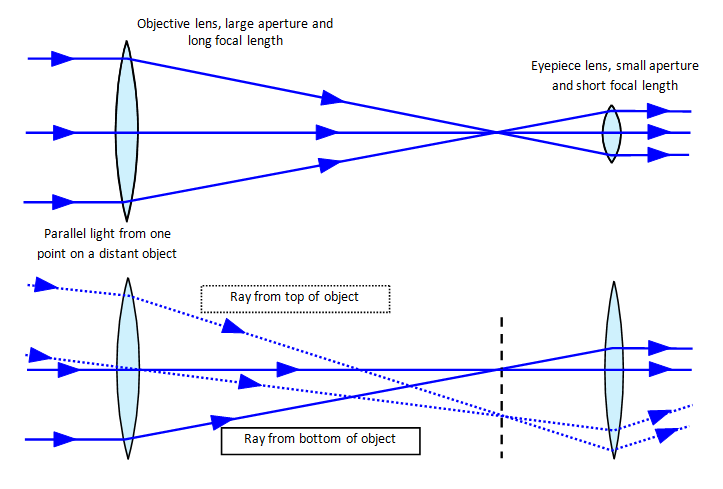
\includegraphics[width= 0.7\textwidth]{images/refractor.png}
    \caption{Refractor Telescope}
    \label{fig:refractor}
\end{figure}
\footnote{Figure \ref{fig:refractor}: Gibbs, Keith, Schoolphysics, \href{https://www.schoolphysics.co.uk/age11-14/Light/text/Telescopes_/index.html}{https://www.schoolphysics.co.uk/age11-14/Light/text/Telescopes\_/index.html}}


    

\FloatBarrier
Code for polar plot (Fornax) (\textbf{Ap.2}):
   \begin{tcolorbox}[breakable, size=fbox, boxrule=1pt, pad at break*=1mm,colback=cellbackground, colframe=cellborder]
\prompt{In}{incolor}{25}{\boxspacing}
\begin{Verbatim}[commandchars=\\\{\}]
\PY{k+kn}{import} \PY{n+nn}{matplotlib}\PY{n+nn}{.}\PY{n+nn}{pyplot} \PY{k}{as} \PY{n+nn}{plt}
\PY{k+kn}{import} \PY{n+nn}{numpy} \PY{k}{as} \PY{n+nn}{np}

\PY{c+c1}{\PYZsh{} Data}
\PY{n}{ra\PYZus{}hours} \PY{o}{=} \PY{p}{[}
    \PY{l+m+mf}{3.3667}\PY{p}{,} \PY{l+m+mf}{2.7717}\PY{p}{,} \PY{l+m+mf}{3.56}\PY{p}{,} \PY{l+m+mf}{3.6089}\PY{p}{,} \PY{l+m+mf}{3.6478}\PY{p}{,} \PY{l+m+mf}{3.4719}\PY{p}{,} \PY{l+m+mf}{3.6478}\PY{p}{,} \PY{l+m+mf}{3.5189}\PY{p}{,} \PY{l+m+mf}{3.3994}\PY{p}{,} \PY{l+m+mf}{3.069}\PY{p}{,} \PY{l+m+mf}{3.6156}\PY{p}{,} \PY{l+m+mf}{3.6008}\PY{p}{,} \PY{l+m+mf}{2.5592}\PY{p}{,} \PY{l+m+mf}{3.6244}\PY{p}{,}
    \PY{l+m+mf}{3.379}\PY{p}{,} \PY{l+m+mf}{2.7289}\PY{p}{,} \PY{l+m+mf}{3.3306}\PY{p}{,} \PY{l+m+mf}{3.5833}\PY{p}{,} \PY{l+m+mf}{3.6089}\PY{p}{,} \PY{l+m+mf}{3.7039}\PY{p}{,} \PY{l+m+mf}{3.2256}\PY{p}{,} \PY{l+m+mf}{3.7053}\PY{p}{,} \PY{l+m+mf}{3.3506}\PY{p}{,} \PY{l+m+mf}{3.2867}\PY{p}{,} \PY{l+m+mf}{2.4189}\PY{p}{,} \PY{l+m+mf}{3.5094}\PY{p}{,} \PY{l+m+mf}{3.5889}\PY{p}{,} \PY{l+m+mf}{3.6122}\PY{p}{,}
    \PY{l+m+mf}{3.4683}\PY{p}{,} \PY{l+m+mf}{3.3042}\PY{p}{,} \PY{l+m+mf}{2.65}\PY{p}{,} \PY{l+m+mf}{3.465}\PY{p}{,} \PY{l+m+mf}{3.5917}\PY{p}{,} \PY{l+m+mf}{3.6183}\PY{p}{,} \PY{l+m+mf}{3.5647}\PY{p}{,} \PY{l+m+mf}{2.8264}\PY{p}{,} \PY{l+m+mf}{2.3517}\PY{p}{,} \PY{l+m+mf}{3.4219}\PY{p}{,} \PY{l+m+mf}{3.4419}\PY{p}{,} \PY{l+m+mf}{3.6744}\PY{p}{,} \PY{l+m+mf}{3.5831}\PY{p}{,} \PY{l+m+mf}{3.1017}\PY{p}{,}
    \PY{l+m+mf}{1.9756}\PY{p}{,} \PY{l+m+mf}{1.9281}\PY{p}{,} \PY{l+m+mf}{3.6692}\PY{p}{,} \PY{l+m+mf}{2.1933}\PY{p}{,} \PY{l+m+mf}{2.6631}\PY{p}{,} \PY{l+m+mf}{1.8214}\PY{p}{,} \PY{l+m+mf}{2.1219}\PY{p}{,} \PY{l+m+mf}{3.3506}\PY{p}{,} \PY{l+m+mf}{3.7839}\PY{p}{,} \PY{l+m+mf}{2.8942}\PY{p}{,} \PY{l+m+mf}{3.1122}\PY{p}{,} \PY{l+m+mf}{3.7064}\PY{p}{,} \PY{l+m+mf}{3.4344}\PY{p}{,} \PY{l+m+mf}{3.4192}\PY{p}{,}
    \PY{l+m+mf}{2.1917}\PY{p}{,} \PY{l+m+mf}{3.16}\PY{p}{,} \PY{l+m+mf}{2.5444}\PY{p}{,} \PY{l+m+mf}{2.6942}\PY{p}{,} \PY{l+m+mf}{2.1144}\PY{p}{,} \PY{l+m+mf}{2.0139}\PY{p}{,} \PY{l+m+mf}{1.7956}\PY{p}{,} \PY{l+m+mf}{3.4806}\PY{p}{,} \PY{l+m+mf}{3.0756}\PY{p}{,} \PY{l+m+mf}{1.8253}\PY{p}{,} \PY{l+m+mf}{2.8664}\PY{p}{,} \PY{l+m+mf}{1.8308}\PY{p}{,} \PY{l+m+mf}{1.8308}\PY{p}{,} \PY{l+m+mf}{3.6353}\PY{p}{,}
    \PY{l+m+mf}{2.0153}\PY{p}{,} \PY{l+m+mf}{1.9567}
\PY{p}{]}
\PY{n}{velocity} \PY{o}{=} \PY{p}{[}
    \PY{l+m+mi}{5209}\PY{p}{,} \PY{l+m+mi}{1261}\PY{p}{,} \PY{l+m+mi}{1650}\PY{p}{,} \PY{l+m+mi}{1877}\PY{p}{,} \PY{l+m+mi}{1942}\PY{p}{,} \PY{l+m+mi}{1182}\PY{p}{,} \PY{l+m+mi}{1398}\PY{p}{,} \PY{l+m+mi}{1902}\PY{p}{,} \PY{l+m+mi}{1371}\PY{p}{,} \PY{l+m+mi}{1695}\PY{p}{,} \PY{l+m+mi}{1296}\PY{p}{,} \PY{l+m+mi}{1324}\PY{p}{,} \PY{l+m+mi}{1942}\PY{p}{,} \PY{l+m+mf}{1498.1}\PY{p}{,} \PY{l+m+mi}{1941}\PY{p}{,} \PY{l+m+mi}{1456}\PY{p}{,} \PY{l+m+mi}{1703}\PY{p}{,} \PY{l+m+mf}{1460.5}\PY{p}{,}
    \PY{l+m+mi}{1724}\PY{p}{,} \PY{l+m+mi}{1510}\PY{p}{,} \PY{l+m+mi}{1686}\PY{p}{,} \PY{l+m+mf}{2022.2}\PY{p}{,} \PY{l+m+mi}{1756}\PY{p}{,} \PY{l+m+mi}{4497}\PY{p}{,} \PY{l+m+mi}{4098}\PY{p}{,} \PY{l+m+mi}{1514}\PY{p}{,} \PY{l+m+mi}{731}\PY{p}{,} \PY{l+m+mi}{1096}\PY{p}{,} \PY{l+m+mi}{1436}\PY{p}{,} \PY{l+m+mi}{1364}\PY{p}{,} \PY{l+m+mi}{1405}\PY{p}{,} \PY{l+m+mi}{1859}\PY{p}{,} \PY{l+m+mi}{1638}\PY{p}{,} \PY{l+m+mi}{1820}\PY{p}{,} \PY{l+m+mi}{1182}\PY{p}{,} \PY{l+m+mi}{6787}\PY{p}{,} \PY{l+m+mi}{4761}\PY{p}{,}
    \PY{l+m+mi}{1371}\PY{p}{,} \PY{l+m+mi}{1436}\PY{p}{,} \PY{l+m+mi}{1714}\PY{p}{,} \PY{l+m+mi}{1368}\PY{p}{,} \PY{l+m+mi}{6196}\PY{p}{,} \PY{l+m+mi}{4559}\PY{p}{,} \PY{l+m+mi}{4356}\PY{p}{,} \PY{l+m+mi}{2022}\PY{p}{,} \PY{l+m+mi}{3506}\PY{p}{,} \PY{l+m+mi}{40}\PY{p}{,} \PY{l+m+mi}{5012}\PY{p}{,} \PY{l+m+mi}{4391}\PY{p}{,} \PY{l+m+mi}{1453}\PY{p}{,} \PY{l+m+mi}{1796}\PY{p}{,} \PY{l+m+mi}{4459}\PY{p}{,} \PY{l+m+mi}{3944}\PY{p}{,} \PY{l+m+mi}{1739}\PY{p}{,} \PY{l+m+mi}{1278}\PY{p}{,} \PY{l+m+mi}{1371}\PY{p}{,}
    \PY{l+m+mi}{6148}\PY{p}{,} \PY{l+m+mi}{3823}\PY{p}{,} \PY{l+m+mi}{1942}\PY{p}{,} \PY{l+m+mi}{4887}\PY{p}{,} \PY{l+m+mi}{5733}\PY{p}{,} \PY{l+m+mi}{4345}\PY{p}{,} \PY{l+m+mi}{8587}\PY{p}{,} \PY{l+m+mi}{1354}\PY{p}{,} \PY{l+m+mi}{6421}\PY{p}{,} \PY{l+m+mi}{7932}\PY{p}{,} \PY{l+m+mi}{6423}\PY{p}{,} \PY{l+m+mi}{4174}\PY{p}{,} \PY{l+m+mi}{8226}\PY{p}{,} \PY{l+m+mi}{882}\PY{p}{,} \PY{l+m+mi}{5420}\PY{p}{,} \PY{l+m+mi}{10887}
\PY{p}{]}

\PY{c+c1}{\PYZsh{} Convert right ascension to radians}
\PY{n}{ra\PYZus{}radians} \PY{o}{=} \PY{n}{np}\PY{o}{.}\PY{n}{deg2rad}\PY{p}{(}\PY{n}{np}\PY{o}{.}\PY{n}{array}\PY{p}{(}\PY{n}{ra\PYZus{}hours}\PY{p}{)} \PY{o}{*} \PY{l+m+mi}{15}\PY{p}{)}

\PY{c+c1}{\PYZsh{} Create polar plot}
\PY{n}{fig} \PY{o}{=} \PY{n}{plt}\PY{o}{.}\PY{n}{figure}\PY{p}{(}\PY{n}{figsize}\PY{o}{=}\PY{p}{(}\PY{l+m+mi}{8}\PY{p}{,} \PY{l+m+mi}{8}\PY{p}{)}\PY{p}{)}
\PY{n}{ax} \PY{o}{=} \PY{n}{fig}\PY{o}{.}\PY{n}{add\PYZus{}subplot}\PY{p}{(}\PY{l+m+mi}{111}\PY{p}{,} \PY{n}{projection}\PY{o}{=}\PY{l+s+s1}{\PYZsq{}}\PY{l+s+s1}{polar}\PY{l+s+s1}{\PYZsq{}}\PY{p}{)}

\PY{c+c1}{\PYZsh{} Plot velocity vs. right ascension}
\PY{n}{ax}\PY{o}{.}\PY{n}{scatter}\PY{p}{(}\PY{n}{ra\PYZus{}radians}\PY{p}{,} \PY{n}{velocity}\PY{p}{,} \PY{n}{c}\PY{o}{=}\PY{l+s+s1}{\PYZsq{}}\PY{l+s+s1}{b}\PY{l+s+s1}{\PYZsq{}}\PY{p}{,} \PY{n}{marker}\PY{o}{=}\PY{l+s+s1}{\PYZsq{}}\PY{l+s+s1}{o}\PY{l+s+s1}{\PYZsq{}}\PY{p}{,} \PY{n}{alpha}\PY{o}{=}\PY{l+m+mf}{0.7}\PY{p}{)}

\PY{c+c1}{\PYZsh{} Set theta (right ascension) tick positions and labels}
\PY{n}{ax}\PY{o}{.}\PY{n}{set\PYZus{}xticks}\PY{p}{(}\PY{n}{np}\PY{o}{.}\PY{n}{linspace}\PY{p}{(}\PY{l+m+mi}{0}\PY{p}{,} \PY{l+m+mi}{2} \PY{o}{*} \PY{n}{np}\PY{o}{.}\PY{n}{pi}\PY{p}{,} \PY{l+m+mi}{12}\PY{p}{,} \PY{n}{endpoint}\PY{o}{=}\PY{k+kc}{False}\PY{p}{)}\PY{p}{)}
\PY{n}{ax}\PY{o}{.}\PY{n}{set\PYZus{}xticklabels}\PY{p}{(}\PY{p}{[}\PY{l+s+s1}{\PYZsq{}}\PY{l+s+s1}{0}\PY{l+s+s1}{\PYZsq{}}\PY{p}{,} \PY{l+s+s1}{\PYZsq{}}\PY{l+s+s1}{2}\PY{l+s+s1}{\PYZsq{}}\PY{p}{,} \PY{l+s+s1}{\PYZsq{}}\PY{l+s+s1}{4}\PY{l+s+s1}{\PYZsq{}}\PY{p}{,} \PY{l+s+s1}{\PYZsq{}}\PY{l+s+s1}{6}\PY{l+s+s1}{\PYZsq{}}\PY{p}{,} \PY{l+s+s1}{\PYZsq{}}\PY{l+s+s1}{8}\PY{l+s+s1}{\PYZsq{}}\PY{p}{,} \PY{l+s+s1}{\PYZsq{}}\PY{l+s+s1}{10}\PY{l+s+s1}{\PYZsq{}}\PY{p}{,} \PY{l+s+s1}{\PYZsq{}}\PY{l+s+s1}{\PYZsq{}}\PY{p}{,} \PY{l+s+s1}{\PYZsq{}}\PY{l+s+s1}{14}\PY{l+s+s1}{\PYZsq{}}\PY{p}{,} \PY{l+s+s1}{\PYZsq{}}\PY{l+s+s1}{16}\PY{l+s+s1}{\PYZsq{}}\PY{p}{,} \PY{l+s+s1}{\PYZsq{}}\PY{l+s+s1}{18}\PY{l+s+s1}{\PYZsq{}}\PY{p}{,} \PY{l+s+s1}{\PYZsq{}}\PY{l+s+s1}{20}\PY{l+s+s1}{\PYZsq{}}\PY{p}{,} \PY{l+s+s1}{\PYZsq{}}\PY{l+s+s1}{22}\PY{l+s+s1}{\PYZsq{}}\PY{p}{]}\PY{p}{)}

\PY{c+c1}{\PYZsh{} Set recessional tick positions and labels}
\PY{n}{max\PYZus{}velocity} \PY{o}{=} \PY{n+nb}{max}\PY{p}{(}\PY{n}{velocity}\PY{p}{)}
\PY{n}{ax}\PY{o}{.}\PY{n}{set\PYZus{}rticks}\PY{p}{(}\PY{n}{np}\PY{o}{.}\PY{n}{linspace}\PY{p}{(}\PY{l+m+mi}{0}\PY{p}{,} \PY{n}{max\PYZus{}velocity}\PY{p}{,} \PY{l+m+mi}{6}\PY{p}{)}\PY{p}{)}
\PY{n}{ax}\PY{o}{.}\PY{n}{set\PYZus{}rlabel\PYZus{}position}\PY{p}{(}\PY{l+m+mf}{22.5}\PY{p}{)}

\PY{c+c1}{\PYZsh{} Adjust recession velocity tick labels}
\PY{n}{ax}\PY{o}{.}\PY{n}{set\PYZus{}rgrids}\PY{p}{(}\PY{n}{np}\PY{o}{.}\PY{n}{linspace}\PY{p}{(}\PY{l+m+mi}{0}\PY{p}{,} \PY{n}{max\PYZus{}velocity}\PY{p}{,} \PY{l+m+mi}{6}\PY{p}{)}\PY{p}{,} \PY{n}{angle}\PY{o}{=}\PY{l+m+mi}{0}\PY{p}{,} \PY{n}{fontsize}\PY{o}{=}\PY{l+m+mi}{10}\PY{p}{,} \PY{n}{ha}\PY{o}{=}\PY{l+s+s1}{\PYZsq{}}\PY{l+s+s1}{left}\PY{l+s+s1}{\PYZsq{}}\PY{p}{)}
\PY{n}{ax}\PY{o}{.}\PY{n}{set\PYZus{}rlabel\PYZus{}position}\PY{p}{(}\PY{l+m+mi}{15}\PY{p}{)}

\PY{c+c1}{\PYZsh{} Set plot title and labels}
\PY{n}{ax}\PY{o}{.}\PY{n}{set\PYZus{}title}\PY{p}{(}\PY{l+s+s1}{\PYZsq{}}\PY{l+s+s1}{Cone Diagram}\PY{l+s+s1}{\PYZsq{}}\PY{p}{,} \PY{n}{fontsize}\PY{o}{=}\PY{l+m+mi}{14}\PY{p}{)}
\PY{n}{ax}\PY{o}{.}\PY{n}{set\PYZus{}xlabel}\PY{p}{(}\PY{l+s+s1}{\PYZsq{}}\PY{l+s+s1}{Right Ascension (hours)}\PY{l+s+s1}{\PYZsq{}}\PY{p}{,} \PY{n}{fontsize}\PY{o}{=}\PY{l+m+mi}{12}\PY{p}{)}
\PY{n}{ax}\PY{o}{.}\PY{n}{set\PYZus{}ylabel}\PY{p}{(}\PY{l+s+s1}{\PYZsq{}}\PY{l+s+s1}{Recession Velocity (km/s)}\PY{l+s+s1}{\PYZsq{}}\PY{p}{,} \PY{n}{fontsize}\PY{o}{=}\PY{l+m+mi}{12}\PY{p}{)}

\PY{c+c1}{\PYZsh{} Show the plot}
\PY{n}{plt}\PY{o}{.}\PY{n}{show}\PY{p}{(}\PY{p}{)}
\end{Verbatim}
\end{tcolorbox}

Code for Fornax Cluster Recessional Velocity \textbf{(Ap.3)}:
\begin{tcolorbox}[breakable, size=fbox, boxrule=1pt, pad at break*=1mm,colback=cellbackground, colframe=cellborder]
\prompt{In}{incolor}{34}{\boxspacing}
\begin{Verbatim}[commandchars=\\\{\}]
\PY{c+c1}{\PYZsh{}Get mean and stanard deviation from velocity list}
\PY{n}{mean} \PY{o}{=} \PY{n}{np}\PY{o}{.}\PY{n}{mean}\PY{p}{(}\PY{n}{velocity}\PY{p}{)}
\PY{n}{std} \PY{o}{=} \PY{n}{np}\PY{o}{.}\PY{n}{std}\PY{p}{(}\PY{n}{velocity}\PY{p}{)}

\PY{c+c1}{\PYZsh{}Create upper and lower thresholds}
\PY{n}{upper} \PY{o}{=} \PY{n}{mean} \PY{o}{+} \PY{p}{(}\PY{l+m+mi}{3} \PY{o}{*} \PY{n}{std}\PY{p}{)} 
\PY{n}{lower} \PY{o}{=} \PY{n}{mean} \PY{o}{\PYZhy{}} \PY{p}{(}\PY{l+m+mi}{3} \PY{o}{*} \PY{n}{std}\PY{p}{)} 

\PY{c+c1}{\PYZsh{}Loop through list to remove any outliers}
\PY{k}{for} \PY{n}{i} \PY{o+ow}{in} \PY{n}{velocity}\PY{p}{:}
    \PY{k}{if}\PY{p}{(}\PY{n}{i} \PY{o}{\PYZgt{}}\PY{o}{=} \PY{n}{upper} \PY{o+ow}{or} \PY{n}{i} \PY{o}{\PYZlt{}}\PY{o}{=} \PY{n}{lower}\PY{p}{)}\PY{p}{:}
        \PY{n}{velocity}\PY{o}{.}\PY{n}{remove}\PY{p}{(}\PY{n}{i}\PY{p}{)}
\end{Verbatim}
\end{tcolorbox}
\begin{tcolorbox}[breakable, size=fbox, boxrule=1pt, pad at break*=1mm,colback=cellbackground, colframe=cellborder]
\prompt{In}{incolor}{34}{\boxspacing}
 \begin{Verbatim}[commandchars=\\\{\}]
[1425,1947,1169,1877,1388,1294,1382,1514,1302,1392,921,1724,1619,1561,\\1418,1323,1740,1373,1613,740,1255,1640,1279,1380,1007,1430,1334,1275,1205,\\1657,1369,1374,1813,1823,2064,1497,808,1856,1189,1980,1138,1660]

Mean: 1783.714
Standard Deviation: 352.526 
    \end{Verbatim}
    \end{tcolorbox}


Data Set for Virgo Cluster Recessional Velocity \textbf{(Ap.4)}:
\begin{tcolorbox}[breakable, size=fbox, boxrule=1pt, pad at break*=1mm,colback=cellbackground, colframe=cellborder]
\prompt{In}{incolor}{34}{\boxspacing}
\begin{Verbatim}[commandchars=\\\{\}]
[997, 1307, 1117, -244, 729, 1060, 1243, 448, 410, 340, 2244, 984, 1210, 532, 1377, 1009, 943, 1730, 801, 1083, 1241, 1142, 950, 843, 1164, 1349, 2273, 1359, 381, 1875, 1609, 1069, 1374, 1375, 967, 561, 1970, 1172, 635, 1071, 875, 1892, 150, 195, 951, 1243, 876, 1871, 2080, 1288, 1084, 567, 1804, 1231, 1881]

Mean: 1061
Standard Deviation: 581 
    \end{Verbatim}
\end{tcolorbox}

















\begin{table}[h!]
    \centering
    \begin{tabular}{c|c}
        VCC 1535 &  0.00149 \\
        VCC 1231 & 0.00749\\
      VCC 1062  &  0.00177 \\
      VCC 1664  &  0.00381 \\
      VCC 944 & 0.00281 \\
       VCC 1279 &  0.00450 \\
       VCC 1025 &  0.00357 \\
       VCC 1475 & 0.00317
    \end{tabular}
    \caption{\textbf{Ap.4} - Virgo Cluster Galaxies' Measured Redshift}
    \label{tab:my_label}
\end{table}


\begin{table}[h!]
    \centering
    \begin{tabular}{c|c}
         FCC 21& 0.00587 \\
         FCC 277& 0.00547 \\
        FCC 55 & 0.00427 \\
        FCC 19 &  0.00499 \\
       FCC 324  &  0.00619 \\
       FCC 288 & 0.00397 \\
       FCC 203  &  0.00380 \\
       NGC 1217  & 0.02067
    \end{tabular}
    \caption{\textbf{Ap.5} - Fornax Cluster Galaxies' Measured Redshift}
    \label{tab:my_label}
\end{table}

\FloatBarrier


\begin{table}[h!]
    \centering
\begin{tabular}{ll}

Galaxy  & Value (\(10^{-8}\)) \\
\hline
VCC 2000 & 5.32600 \\
VCC 1720 & 5.19510 \\
VCC 1729 & 5.51343 \\
VCC 369  & 5.41072 \\
VCC 1154 & 5.45181 \\
VCC 828  & 5.80018 \\
VCC 1475 & 5.16841 \\
VCC 1535 & 4.50943 \\
\hline
\end{tabular}
    \caption{\textbf{Ap.6} - Virgo Cluster Parallax Angles}
    \label{tab:my_label}
\end{table}
\FloatBarrier
\begin{table}[h!]
    \centering
    \begin{tabular}{c|c}
Galaxy  & Value (\(10^{-8}\)) \\
\hline
FCC 47   & 5.431 \\
FCC 170  & 5.431 \\
FCC 83   & 6.833\\
FCC 301  & 5.917 \\
FCC 324* & 6.596 \\
FCC 288* & 7.222 \\
NGC 1217*& 6.492 \\
NGC 854  & 6.418 \\
\hline
\end{tabular}
    \caption{\textbf{Ap.7} - Fornax Cluster Parallax Angles}
    \label{tab:my_label}
\end{table}

\newpage
\textcolor{white}{h}
\newpage
\newpage
\FloatBarrier
\bibliographystyle{plain}
\bibliography{refs}
\end{document}



